



\documentclass[
	% -- opções da classe memoir --
	12pt,				% tamanho da fonte
	openright,			% capítulos começam em pág ímpar (insere página vazia caso preciso)
	oneside,			% para impressão em recto e verso. Oposto a oneside
	a4paper,			% tamanho do papel. 
	% -- opções da classe abntex2 --
	%chapter=TITLE,		% títulos de capítulos convertidos em letras maiúsculas
	%section=TITLE,		% títulos de seções convertidos em letras maiúsculas
	%subsection=TITLE,	% títulos de subseções convertidos em letras maiúsculas
	%subsubsection=TITLE,% títulos de subsubseções convertidos em letras maiúsculas
	% -- opções do pacote babel --
	english,			% idioma adicional para hifenização
	french,				% idioma adicional para hifenização
	spanish,			% idioma adicional para hifenização
	brazil				% o último idioma é o principal do documento
	]{abntex2}




% Pacotes básicos 
\usepackage{lmodern}			% Usa a fonte Latin Modern			
\usepackage[T1]{fontenc}		% Selecao de codigos de fonte.
\usepackage[utf8]{inputenc}		% Codificacao do documento (conversão automática dos acentos)
\usepackage{indentfirst}		% Indenta o primeiro parágrafo de cada seção.
\usepackage{color}				% Controle das cores
\usepackage{graphicx}			% Inclusão de gráficos
\usepackage{microtype} 			% para melhorias de justificação
\usepackage{amsmath}			% lib para equacoes
\usepackage{svg}
%\usepackage{float}
\usepackage[T1]{fontenc}
\usepackage{listings}
\usepackage{tikz}
\usepackage{caption}
\usetikzlibrary{shapes.geometric, arrows}

\tikzstyle{startstop} = [rectangle, rounded corners, 
minimum width=3cm, 
minimum height=1cm,
text centered, 
draw=black, 
fill=red!30]

\tikzstyle{io} = [trapezium, 
trapezium stretches=true, % A later addition
trapezium left angle=70, 
trapezium right angle=110, 
minimum width=3cm, 
minimum height=1cm, text centered, 
draw=black, fill=blue!30]


\tikzstyle{process} = [rectangle, 
minimum width=3cm, 
minimum height=1cm, 
text centered, 
text width=3cm, 
draw=black, 
fill=orange!30]

\tikzstyle{decision} = [diamond, 
minimum width=3cm, 
minimum height=1cm, 
text centered, 
draw=black, 
fill=green!30]
\tikzstyle{arrow} = [thick,->,>=stealth]



\definecolor{dkgreen}{rgb}{0,0.6,0}
\definecolor{gray}{rgb}{0.5,0.5,0.5}
\definecolor{mauve}{rgb}{0.58,0,0.82}

\lstset{frame=tb,
  language=Python,
  aboveskip=3mm,
  belowskip=3mm,
  showstringspaces=false,
  columns=flexible,
  basicstyle={\small\ttfamily},
  numbers=none,
  numberstyle=\tiny\color{gray},
  keywordstyle=\color{blue},
  commentstyle=\color{dkgreen},
  stringstyle=\color{mauve},
  breaklines=false,
  breakatwhitespace=false,
  upquote=true,
  tabsize=3
}

% Pacotes adicionais, usados apenas no âmbito do Modelo Canônico do abnteX2

\usepackage{lipsum}				% para geração de dummy text



% Pacotes de citações
\usepackage[num, backend=biblatex]{abntex2cite}	% Citações padrão ABNT
\usepackage[brazilian,hyperpageref]{backref}	 % Paginas com as citações na bibl


 
% CONFIGURAÇÕES DE PACOTES

% Configurações do pacote backref
% Usado sem a opção hyperpageref de backref
\renewcommand{\backrefpagesname}{Citado na(s) página(s):~}
% Texto padrão antes do número das páginas
\renewcommand{\backref}{}
% Define os textos da citação
\renewcommand*{\backrefalt}[4]{
	\ifcase #1 %
		Nenhuma citação no texto.%
	\or
		Citado na página #2.%
	\else
		Citado #1 vezes nas páginas #2.%
	\fi}%
% ---



% ---
% Informações de dados para CAPA e FOLHA DE ROSTO
% ---
\titulo{Robô omnidirecional de 3 rodas}
\autor{Daniel Ermelino Carvalho \\ Lucas Pereira Lima}
\local{Brasil}
\data{2024}
\orientador{Marcelo Bender Perotoni}
\instituicao{%
  Universidade Federal do ABC
  \par
  CECS
  \par
   Engenharia de Instrumentação, Automação e Robótica}
\tipotrabalho{Tese (Doutorado)}
% O preambulo deve conter o tipo do trabalho, o objetivo, 
% o nome da instituição e a área de concentração 
\preambulo{ }



% Configurações de aparência do PDF final

% alterando o aspecto da cor azul
\definecolor{blue}{RGB}{5,5,180}

% informações do PDF
\makeatletter
\hypersetup{
     	%pagebackref=true,
		pdftitle={\@title}, 
		pdfauthor={\@author},
    	pdfsubject={\imprimirpreambulo},
	    pdfcreator={LaTeX with abnTeX2},
		pdfkeywords={abnt}{latex}{abntex}{abntex2}{trabalho acadêmico}, 
		colorlinks=true,       		% false: boxed links; true: colored links
    	linkcolor=blue,          	% color of internal links
    	citecolor=blue,        		% color of links to bibliography
    	filecolor=magenta,      		% color of file links
		urlcolor=blue,
		bookmarksdepth=4
}
\makeatother


% Posiciona figuras e tabelas no topo da página quando adicionadas sozinhas
% em um página em branco. Ver https://github.com/abntex/abntex2/issues/170
\makeatletter
\setlength{\@fptop}{5pt} % Set distance from top of page to first float
\makeatother



% Possibilita criação de Quadros e Lista de quadros.
% Ver https://github.com/abntex/abntex2/issues/176

\newcommand{\quadroname}{Quadro}
\newcommand{\listofquadrosname}{Lista de quadros}

\newfloat[chapter]{quadro}{loq}{\quadroname}
\newlistof{listofquadros}{loq}{\listofquadrosname}
\newlistentry{quadro}{loq}{0}

% configurações para atender às regras da ABNT
\setfloatadjustment{quadro}{\centering}
\counterwithout{quadro}{chapter}
\renewcommand{\cftquadroname}{\quadroname\space} 
\renewcommand*{\cftquadroaftersnum}{\hfill--\hfill}

\setfloatlocations{quadro}{hbtp} % Ver https://github.com/abntex/abntex2/issues/176



% Espaçamentos entre linhas e parágrafos 


% O tamanho do parágrafo é dado por:
\setlength{\parindent}{1.3cm}

% Controle do espaçamento entre um parágrafo e outro:
\setlength{\parskip}{0.2cm}  % tente também \onelineskip


% compila o indice
\makeindex




% Início do documento
\begin{document}

% Seleciona o idioma do documento (conforme pacotes do babel)
%\selectlanguage{english}
\selectlanguage{brazil}

% Retira espaço extra obsoleto entre as frases.
\frenchspacing 


% ELEMENTOS PRÉ-TEXTUAIS
	
% ---
% Capa
% ---
\imprimircapa
% ---

% ---
% Folha de rosto
% (o * indica que haverá a ficha bibliográfica)
% ---
\imprimirfolhaderosto
% ---


% ---
% RESUMOS
% ---

% resumo em português
\setlength{\absparsep}{18pt} % ajusta o espaçamento dos parágrafos do resumo
\begin{resumo}
 Segundo a , o resumo deve ressaltar o
 objetivo, o método, os resultados e as conclusões do documento. A ordem e a extensão
 destes itens dependem do tipo de resumo (informativo ou indicativo) e do
 tratamento que cada item recebe no documento original. O resumo deve ser
 precedido da referência do documento, com exceção do resumo inserido no
 próprio documento. (\ldots) As palavras-chave devem figurar logo abaixo do
 resumo, antecedidas da expressão Palavras-chave:, separadas entre si por
 ponto e finalizadas também por ponto.

 \textbf{Palavras-chave}: latex. abntex. editoração de texto.
\end{resumo}

% resumo em inglês
\begin{resumo}[Abstract]
 \begin{otherlanguage*}{english}
   This is the english abstract.

   \vspace{\onelineskip}
 
   \noindent 
   \textbf{Keywords}: latex. abntex. text editoration.
 \end{otherlanguage*}
\end{resumo}


% ---
% inserir lista de ilustrações
% ---
\pdfbookmark[0]{\listfigurename}{lof}
\listoffigures*
\cleardoublepage
% ---

% ---
% inserir lista de quadros
% ---
\pdfbookmark[0]{\listofquadrosname}{loq}
\listofquadros*
\cleardoublepage
% ---

% ---
% inserir lista de tabelas
% ---
\pdfbookmark[0]{\listtablename}{lot}
\listoftables*
\cleardoublepage
% ---

% ---
% inserir lista de abreviaturas e siglas
% ---
\begin{siglas}
  \item[ABNT] Associação Brasileira de Normas Técnicas
  \item[abnTeX] ABsurdas Normas para TeX
\end{siglas}
% ---

% ---
% inserir lista de símbolos
% ---
\begin{simbolos}
  \item[$ \omega $] Letra grega minúscula ômega
  \item[$ \theta $] Letra grega minúscula theta
\end{simbolos}
% ---

% ---
% inserir o sumario
% ---
\pdfbookmark[0]{\contentsname}{toc}
\tableofcontents*
\cleardoublepage
% ---


% ELEMENTOS TEXTUAIS
\textual

	% Introdução (exemplo de capítulo sem numeração, mas presente no Sumário)
	\chapter{Introdução}

	

Apesar dos diversos desenvolvimentos recentes, pesquisas no campo da robótica móvel são um fenômeno ocorrendo há mais de 50 anos - segundo os padrões atuais, 
o primeiro robô móvel foi o Shakey, desenvolvido entre 1966 e 1972 \cite{TAKAHASHI}. 
Sua principal característica distintiva era a habilidade de perceber arrazoar a respeito de seu entorno, 
sendo capaz de desenvolver tarefas que requeressem planejamento, encontrar rotas e reposicionar pequenos objetos \cite{sri_international}.

À medida em que as técnicas para se construir e controlar robôs móveis (com particular interesse nos robôs móveis autônomos), 
e a isso se somando o fato de que os materias para sua construção tornaram-se cada vez mais acessíveis (em termos de disponibilidade 
e também de redução de custos), já a partir da década de 80 começaram a surgir robôs autônomos em diversos laboratórios e centros de pesquisa;
 mais recentemente, empresas começaram a comercializar robôs para usuários domésticos, em aplicações como cortadores de grama, aspiradores e pó, 
 e mesmo robôs voltados para entretenimento \cite{TAKAHASHI}.

Robôs são classificáveis diversas maneiras, tais como forma de movimentação, os tipos de tarefas executadas e o seu grau de autonomia, 
bem como agrupando-os entre aquáticos, aéreos e terrestres. A escolha de um dado sistema de locomoção depende de diversas características do robô e 
da tarefa a ser executada, como manobrabilidade, controlabilidade, estabilidade, eficiência e tração \cite{TAKAHASHI}.

Ao se classificar robôs móveis, também é possível se empregar como critério características cinemáticas - particularmente, 
a capacidade do robô se movimentar em qualquer direção. A robôs com restrições em determinados tipos de movimento dá-se o nome de não-holonômicos, 
em oposição a robôs holonômicos, capazes de movimentação em qualquer direção (estritamente, robôs com quantidades de velocidades igual a seu grau de liberdade \cite{TAKAHASHI}).

Em se tratando de robôs terrestres, suas restrições não-holonômicas são consequência direta das rodas empregadas em sua construções. 
Rodas convencionais permitem uma quantidade de movimentos limitada, e, para contornar isso, é possível construir rodas omnidirecionais aos se acrescentar rotores à estrutura de uma roda convencional \cite{TAKAHASHI}.


	% Capitulo com exemplos de comandos inseridos de arquivo externo 
	\include{abntex2-modelo-include-comandos}
	
	\chapter{Objetivos}

\subsection*{Gerais}
Este trabalho tem como objetivos gerais avaliar a viabilidade da utilização de 
um robô omnidirecional de três rodas controlado por microcontrolador para 
atuação independente em ambiente interno.

\subsection*{Específicos}
Deseja-se realizar a construção de um robô a partir de diversos componentes 
(motor, microcontrolador, rodas, driver, chassi, entre outros), e também 
implementar rotina de controle que permita ao robô receber como entrada mapa
do ambiente em que se encontra, de modo que seja capaz de nele se mover de 
acordo com as rotinas desejadas.

	
\chapter{Revisão Bibliográfica}


\section{Veículo omnidirecional de 3 rodas}

Um veículo omnidirecional de 3 rodas no contexto deste trabalho é um robô
holonômico capaz de se mover em translação e rotação simultaneamente e
independentemente \cite{mobile_manipulator_robot}. Sua geometria básica se 
baseia em rodas equidistantes em uma circunferência, com 120° de separação entre
 si, tangenciando o perímetro do chassi do veículo.

\begin{figure}[h]
	\centering
	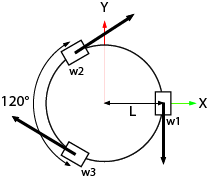
\includegraphics{figures/model}
	\caption{Diagrama do modelo matemático do robô}
\end{figure}


\subsection{Modelagem Cinemática - Dedução da matriz por cinemática direta}

$\overrightarrow{V}$ é o vetor de velocidade linear do robô, $V_{w1}$, $V_{w2}$,
$V_{w3}$ são as velocidades lineares das rodas 1,2,3. 
$\omega $ é a velocidade angular do robô a partir do centro geométrico do robô.
$L$ é a distância entre o centro de geométrico da roda e o centro de geométrico
do robô.


\begin{figure}[h]
	\centering
	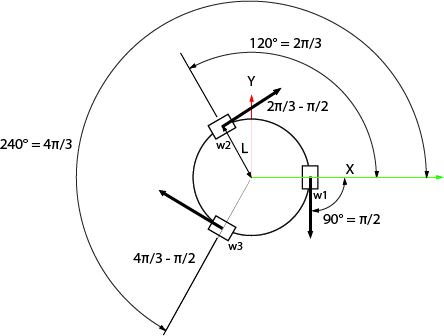
\includegraphics[width=0.9\textwidth]{figures/digram_model_dedution}
	\caption{Diagrama do modelo matemático do robô, com valores dos ângulos das rodas}
\end{figure}

\begin{equation}
    \begin{split}
        \overrightarrow{V}_{l} = 
        \overrightarrow{V}_{w1}
        + \overrightarrow{V}_{w2}
        + \overrightarrow{V}_{w3}
    \end{split}
\end{equation}

\begin{equation}
    \begin{split}
        \overrightarrow{\omega} = 
        \frac{\vert\overrightarrow{V}_{w1}\vert}{L}
        + \frac{\vert\overrightarrow{V}_{w2}\vert}{L}
        + \frac{\vert\overrightarrow{V}_{w3}\vert}{L}
    \end{split}
\end{equation}


\begin{gather*}
        V_{l} \angle \theta =  
        V_{w1} \angle \left(-\frac{\pi}{2}\right) 
        + V_{w2} \angle \left(\frac{2\pi}{3}-\frac{\pi}{2}\right) 
        + V_{w3} \angle \left(\frac{4\pi}{3}-\frac{\pi}{2}\right) 
\end{gather*}

\begin{align*}
    V_{l} \cos{ \theta } + jV_{l} \sin{\theta} =  
    V_{w1} \cos{ \left(-\frac{\pi}{2}\right)} + jV_{w1} \sin{ \left(-\frac{\pi}{2}\right) } \\
    + V_{w2}  \cos{ \left(\frac{\pi}{6}\right) } + jV_{w2}  \sin{ \left(\frac{\pi}{6}\right) }  \\
    + V_{w3} \cos{ \left(\frac{5\pi}{6}\right) } + jV_{w2}  \sin{ \left(\frac{5\pi}{6}\right) } 
\end{align*}

\begin{equation*}
    \begin{split}
        \omega = 
        \frac{V_{w1}}{L}
        + \frac{V_{w2}}{L}
        + \frac{V_{w3}}{L}
    \end{split}
\end{equation*}


\begin{gather}
	\begin{bmatrix} V\cdot \cos{\theta} \\  V\cdot \sin{\theta} \\  \omega \end{bmatrix}
	=
	\begin{bmatrix}
		\cos{\left(-\frac{\pi}{2}\right)} & \cos{\left(\frac{\pi}{6}\right)} & \cos{\left(\frac{5\pi}{6}\right)} \\
		\sin{\left(-\frac{\pi}{2}\right)} & \sin{\left(\frac{\pi}{6}\right)} & \sin{\left(\frac{5\pi}{6}\right)} \\
		\frac{1}{L} & \frac{1}{L} & \frac{1}{L}
	\end{bmatrix}
	\cdot
	\begin{bmatrix} V_{w1} \\  V_{w2} \\  V_{w3} \end{bmatrix}
\end{gather}


Matriz da cinemática direta.

\begin{gather}
	\begin{bmatrix}
		\cos{\left(-\frac{\pi}{2}\right)} & \cos{\left(\frac{\pi}{6}\right)} & \cos{\left(\frac{5\pi}{6}\right)} \\
		\sin{\left(-\frac{\pi}{2}\right)} & \sin{\left(\frac{\pi}{6}\right)} & \sin{\left(\frac{5\pi}{6}\right)} \\
		\frac{1}{L} & \frac{1}{L} & \frac{1}{L}
	\end{bmatrix}
	=
	\begin{bmatrix}
		0 & \sqrt{3}/2 & -\sqrt{3}/2 \\
		1 & -1/2 & -1/2  \\
		1/L & 1/L & 1/L
	\end{bmatrix}
\end{gather}



Matriz inversa?


\begin{gather}
	\begin{bmatrix} V_{w1} \\  V_{w2} \\  V_{w3} \end{bmatrix}
	=
	\begin{bmatrix}
		0 & 2/3 & L/3 \\
		-1/\sqrt{3} & -1/3 & L/3\\
		1/\sqrt{3} & -1/3 & L/3
	\end{bmatrix}
	\cdot
	\begin{bmatrix} V\cdot \cos{\theta} \\  V\cdot \sin{\theta} \\  \omega \end{bmatrix}
\end{gather}


A matriz gerada acima é a matriz de cinemática do robô.
As entradas são o vetor velocidade linear e a velocidade angular do robô, e as
saídas são as velocidades lineares de cada uma das rodas.

Desconsiderando a velocidade angular, é possível observar os vetores velocidades
 das rodas e o vetor velocidade linear do robô na figura \ref{simulacao} que foi
 gerada por meio de simulação em Python.

\begin{figure}[h]
	\centering
	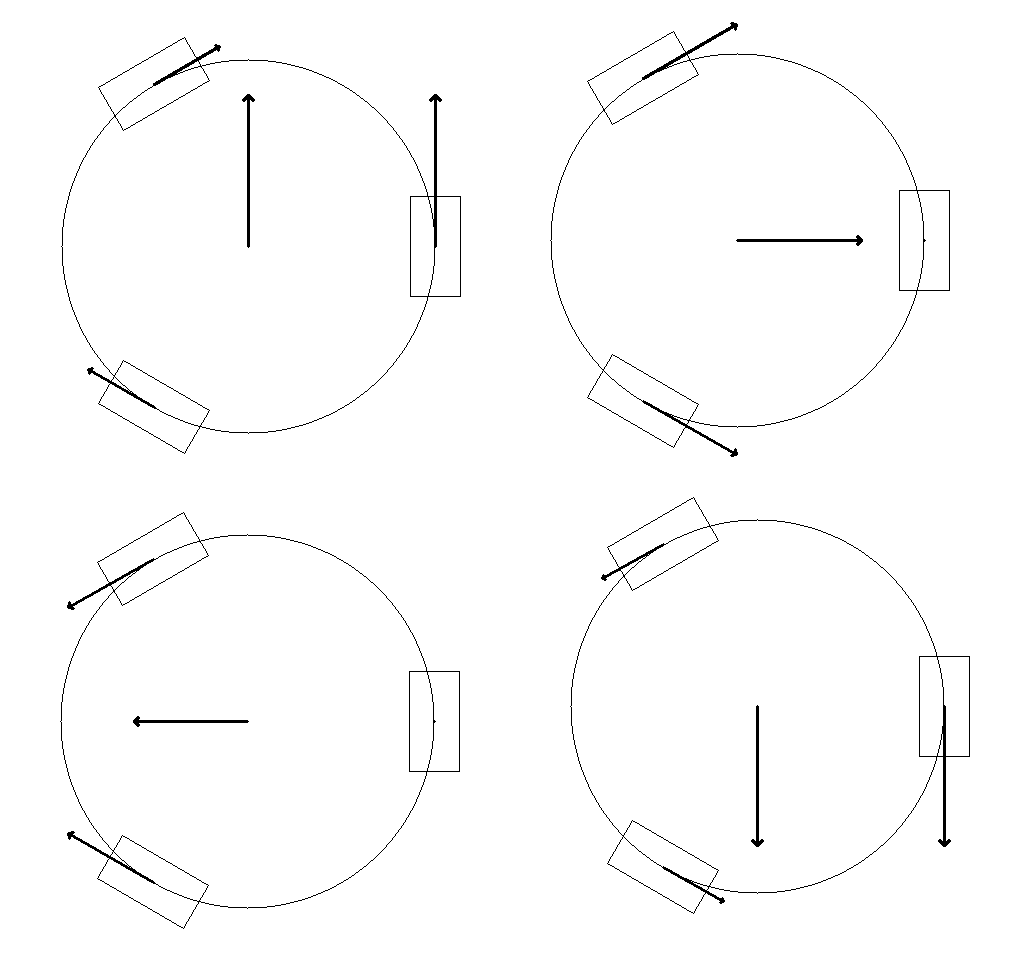
\includegraphics[width=0.7\textwidth]{figures/simulacao}
	\caption{Simulação dos vetores}
	\label{simulacao}
\end{figure}

\section{Roda Omnidirecional}
A roda omnidirecional aparece em vários modelos na literatura, como exemplo o design feito por J. Graboweicki em 1919 \cite{patent_US1305535A}
o design feito por Josef Blumrich em 1972 \cite{patent_US3789947A}.
A roda consiste em rolos perpendiculares (90°) a direção de giro da roda,o efeito é sua capacidade da roda se mover em mais de uma direção ao mesmo tempo.

\begin{figure}[h]
	\centering
	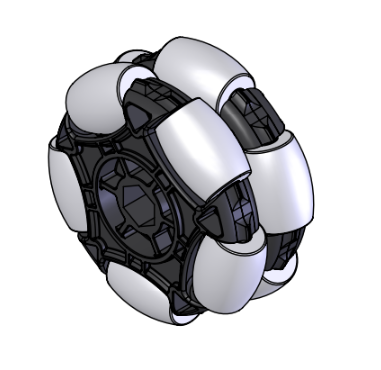
\includegraphics{figures/omniwheel}
	\caption{Modelo de uma Omniwheel \cite{draw_omniwheel}}
\end{figure}

A relação entre velocidade linear e angular da roda, se da por:

\[V_{w1} = \omega_{w1}\cdot r \] 

$V_{w}$ é velocidade linear da roda, $r$ raio da roda, $\omega_{w} $ é a velocidade angular da roda.


Uma variação da roda omnidirecional é a roda mecanum, inventada por Bengt Ilon \cite{patent_US3876255A}, que possue rolos em 45°.



\section{Motor DC com encoder e driver para motor}

Um motor DC é basicamente uma máquina elétrica de corrente contínua, que converte energia elétrica de corrente contínua em energia mecânica
Máquinas elétricas CC são mais fácies de controlar e oferecem uma grande faixa de velocidades \cite{Maquinas_eletricas}.
Devido a sua facilidade de controle, se tornam ótimos canditados para uso em eletrónica e robótica, pois podem ser usados com baterias
Para controlar a velocidade de um motor, é necessário o uso de um encoder, que converte o sinal de posição em um valor medível de velocidade angular.


O motor a ser usado será um motor DC de 6V 210rpm, com taxa de redução de 1:34
O encoder a ser usado nesse projeto é um encoder magnético, que já vem montado no motor a ser usado, com 11 PPR (Pulses Per Revolution).

\subsection{Encoder magnético}

Por ser um encoder PRR, ele produz duas ondas quadradas como saídas, A e B \cite{encoder_ppr}.
As duas possui 90° de fase em si, e se a onda A estiver adiantada em relação a onda B, o sentido de rotação é positivo (contra o relógio)

\begin{figure}[h]
	\centering
	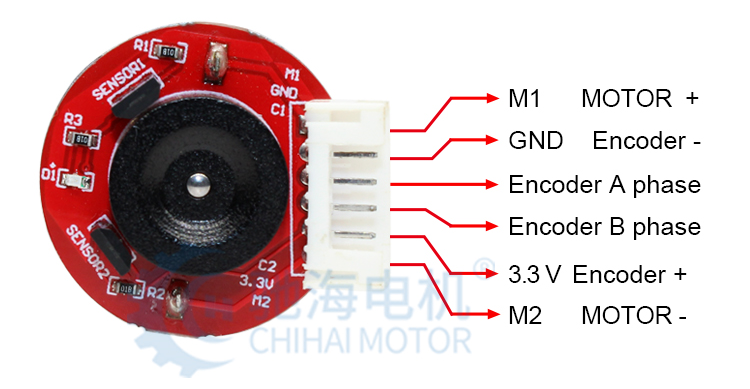
\includegraphics[width=0.6\textwidth]{figures/encoder_holzer}
	\caption{Encoder holzer \cite{encoder_holzer}}
\end{figure}

\begin{figure}[h]
	\centering
	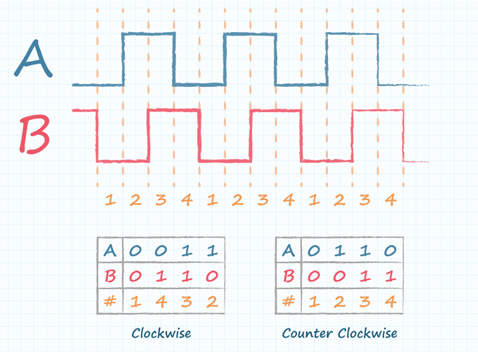
\includegraphics[width=0.7\textwidth]{figures/encoder_pulso_ab}
	\caption{Ondas quadradas resultantes dos pulsos de saída do encoder \cite{encoder_ppr}}
\end{figure}




\section{Microcontrolador STM32}


Microcontroladores são circuitos integrados compactos desenvolvidos para governar
uma operação específica em um sistema embarcado. No contexto da aplicação deste
trabalho, o uso de um microcontrolador é fundamental para se obter o controle
desejado de trajetória e posicionamento do robô.

\subsection{STM32 - STM32F103C8}

STM32 é uma família de microcontroladores de 32-bits fabricados pela
ST-Microelectronics. O processador empregado nessa família é o ARM Cortex-M3 (\cite{cortex_m3}),
baseado em arquitetura Harvard, de 32-bits. Os microcontroladores STM32 fornecem
base para uma uma grande variedades de sistemas embarcados, com custo inferior
e maior flexibilidade quando comparado ao Arduino com ATmega, que possui
microcontroladores de 8 a 16 bits. Contudo, essa flexibilidade e baixo custo têm
como contrapartida o requerimento de um maior nível de experiência em
programação C do que o necessário para desenvolver as mesmas soluções em
Arduino (cuja concepção teve como objetivo maior acessibilidade para iniciantes
em programação em geral, e também  em desenvolvimento de aplicações com
microcontroladores.

O STM32F103C8 (abreviado como STM32 ao longo deste trabalho),
também conhecido como Blue Pill. Tem 64Kbs de memória flash.  De acordo com o \textit{livro Discovering the STM32 Microcontroller} (\cite{stm_doc}) e 
a documentação colaborativa (\cite{stm32_base_org}) do projeto STM32-base (\cite{stm32_base}),
possui também 7 timers, 2 ADCs, e 9 interfaces de comunicação, incluindo I2C (\textit{Inter-Integrated Circuit}), USART 
\textit{Universal Synchronous Asynchronous Receiver Transmitter}), SPI (\textit{Serial Peripheral Interface}), CAN e
USB 2.0. O STM32 apresenta 7 pinos que suportam canais de PWM de 5V, e outros 8 canais de 3.3V, e pode ser alimentado
via microUSB de 5V. Existem 3 grupos de pinos,  $P_{A}$,  $P_{B}$ e  $P_{C}$: os pinos PA vão de $P_{A0}$ 
a $P_{A15}$, PB indo de $P_{B0}$ a $P_{B15}$, e PC com apenas 3 pinos, $P_{C13}$, $P_{C14}$ e $P_{C15}$.
A relação geral dos pinos pode ser melhor obervada na figura \ref{stm32f103c8_pinout}.

\begin{figure}[htb]
	\centering
	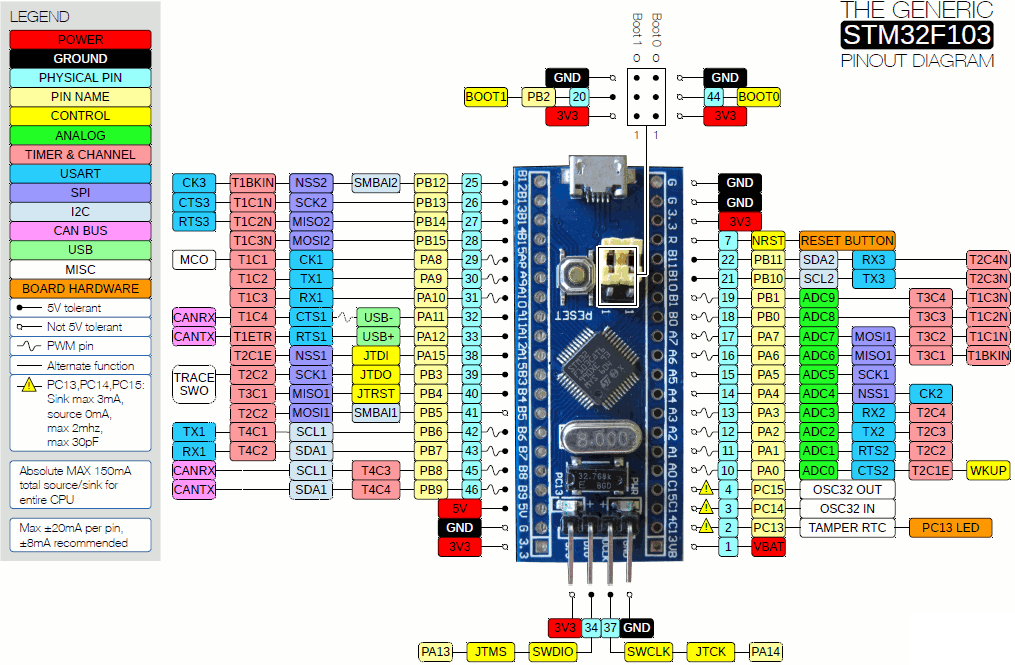
\includegraphics[width=1.0\textwidth]{figures/stm32f1_pinout}
	\caption{Diagrama de pinos do STM32F103C8}
    \label{stm32f103c8_pinout}
\end{figure}

Para carregar o projeto no microcontrolador, tem por padrão o uso do gravador ST-LINK v2.
O ST-link, cujo original (figura \ref{stlinkv2_original}) é fabricado pela ST-Microelectronics \cite{st_link_v2}, 
possui uma versão paralela mais barata
comercializada online (figura \ref{stlinkv2_cheap}), porém a versão paralelo costuma ter fabricantes diversos e 
muitas vezes não descritos na distribuição do produto 
e a relação de pinos pode variar (figura \ref{stlinkv2_cheap_pin_diff}).


\begin{figure}[htb]
	\centering
	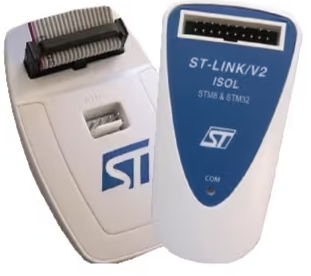
\includegraphics[width=0.5\textwidth]{figures/stlinkv2_original}
	\caption{St-Link V2 original fabricado pela ST-Microelectronics \cite{st_link_v2}}
    \label{stlinkv2_original}
\end{figure}


\begin{figure}[htb]
	\centering
	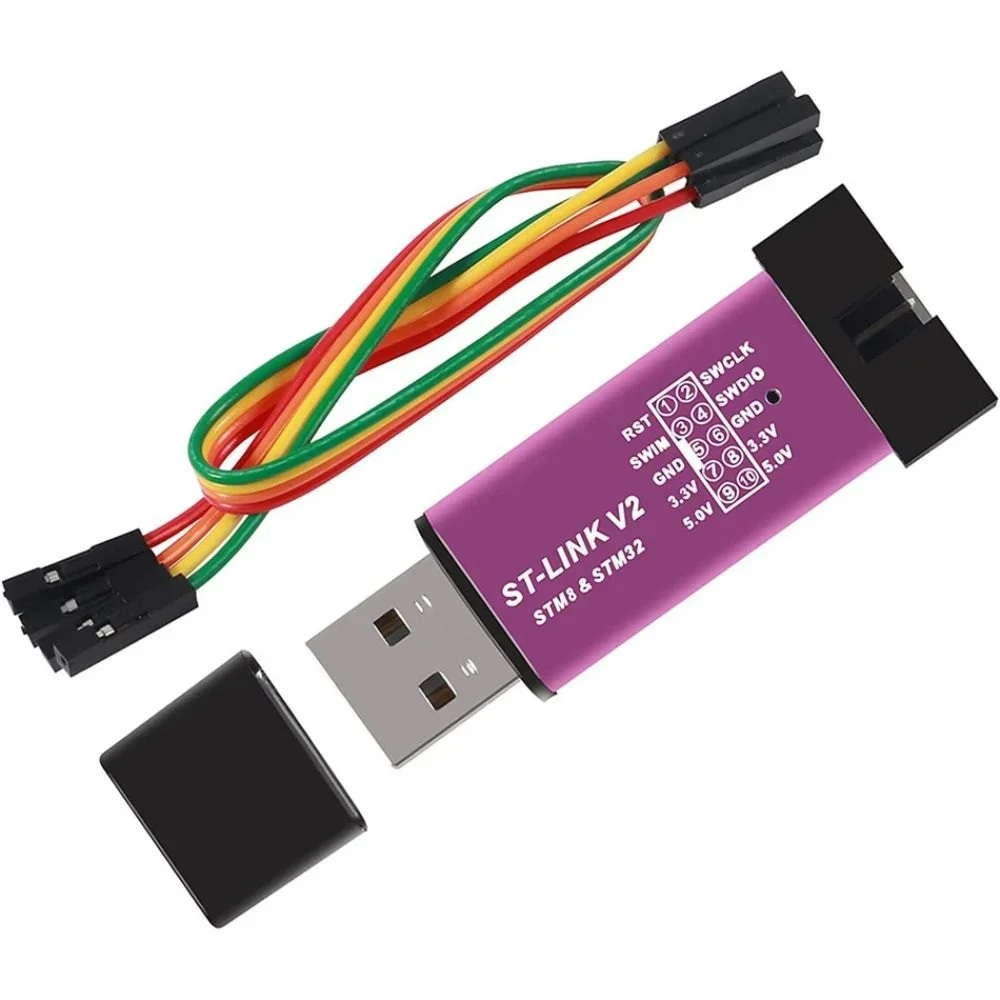
\includegraphics[width=0.5\textwidth]{figures/stlinkv2_cheap}
	\caption{St-Link V2 paralelo de fabricação desconhecida}
    \label{stlinkv2_cheap}
\end{figure}


\begin{figure}[htb]
	\centering
	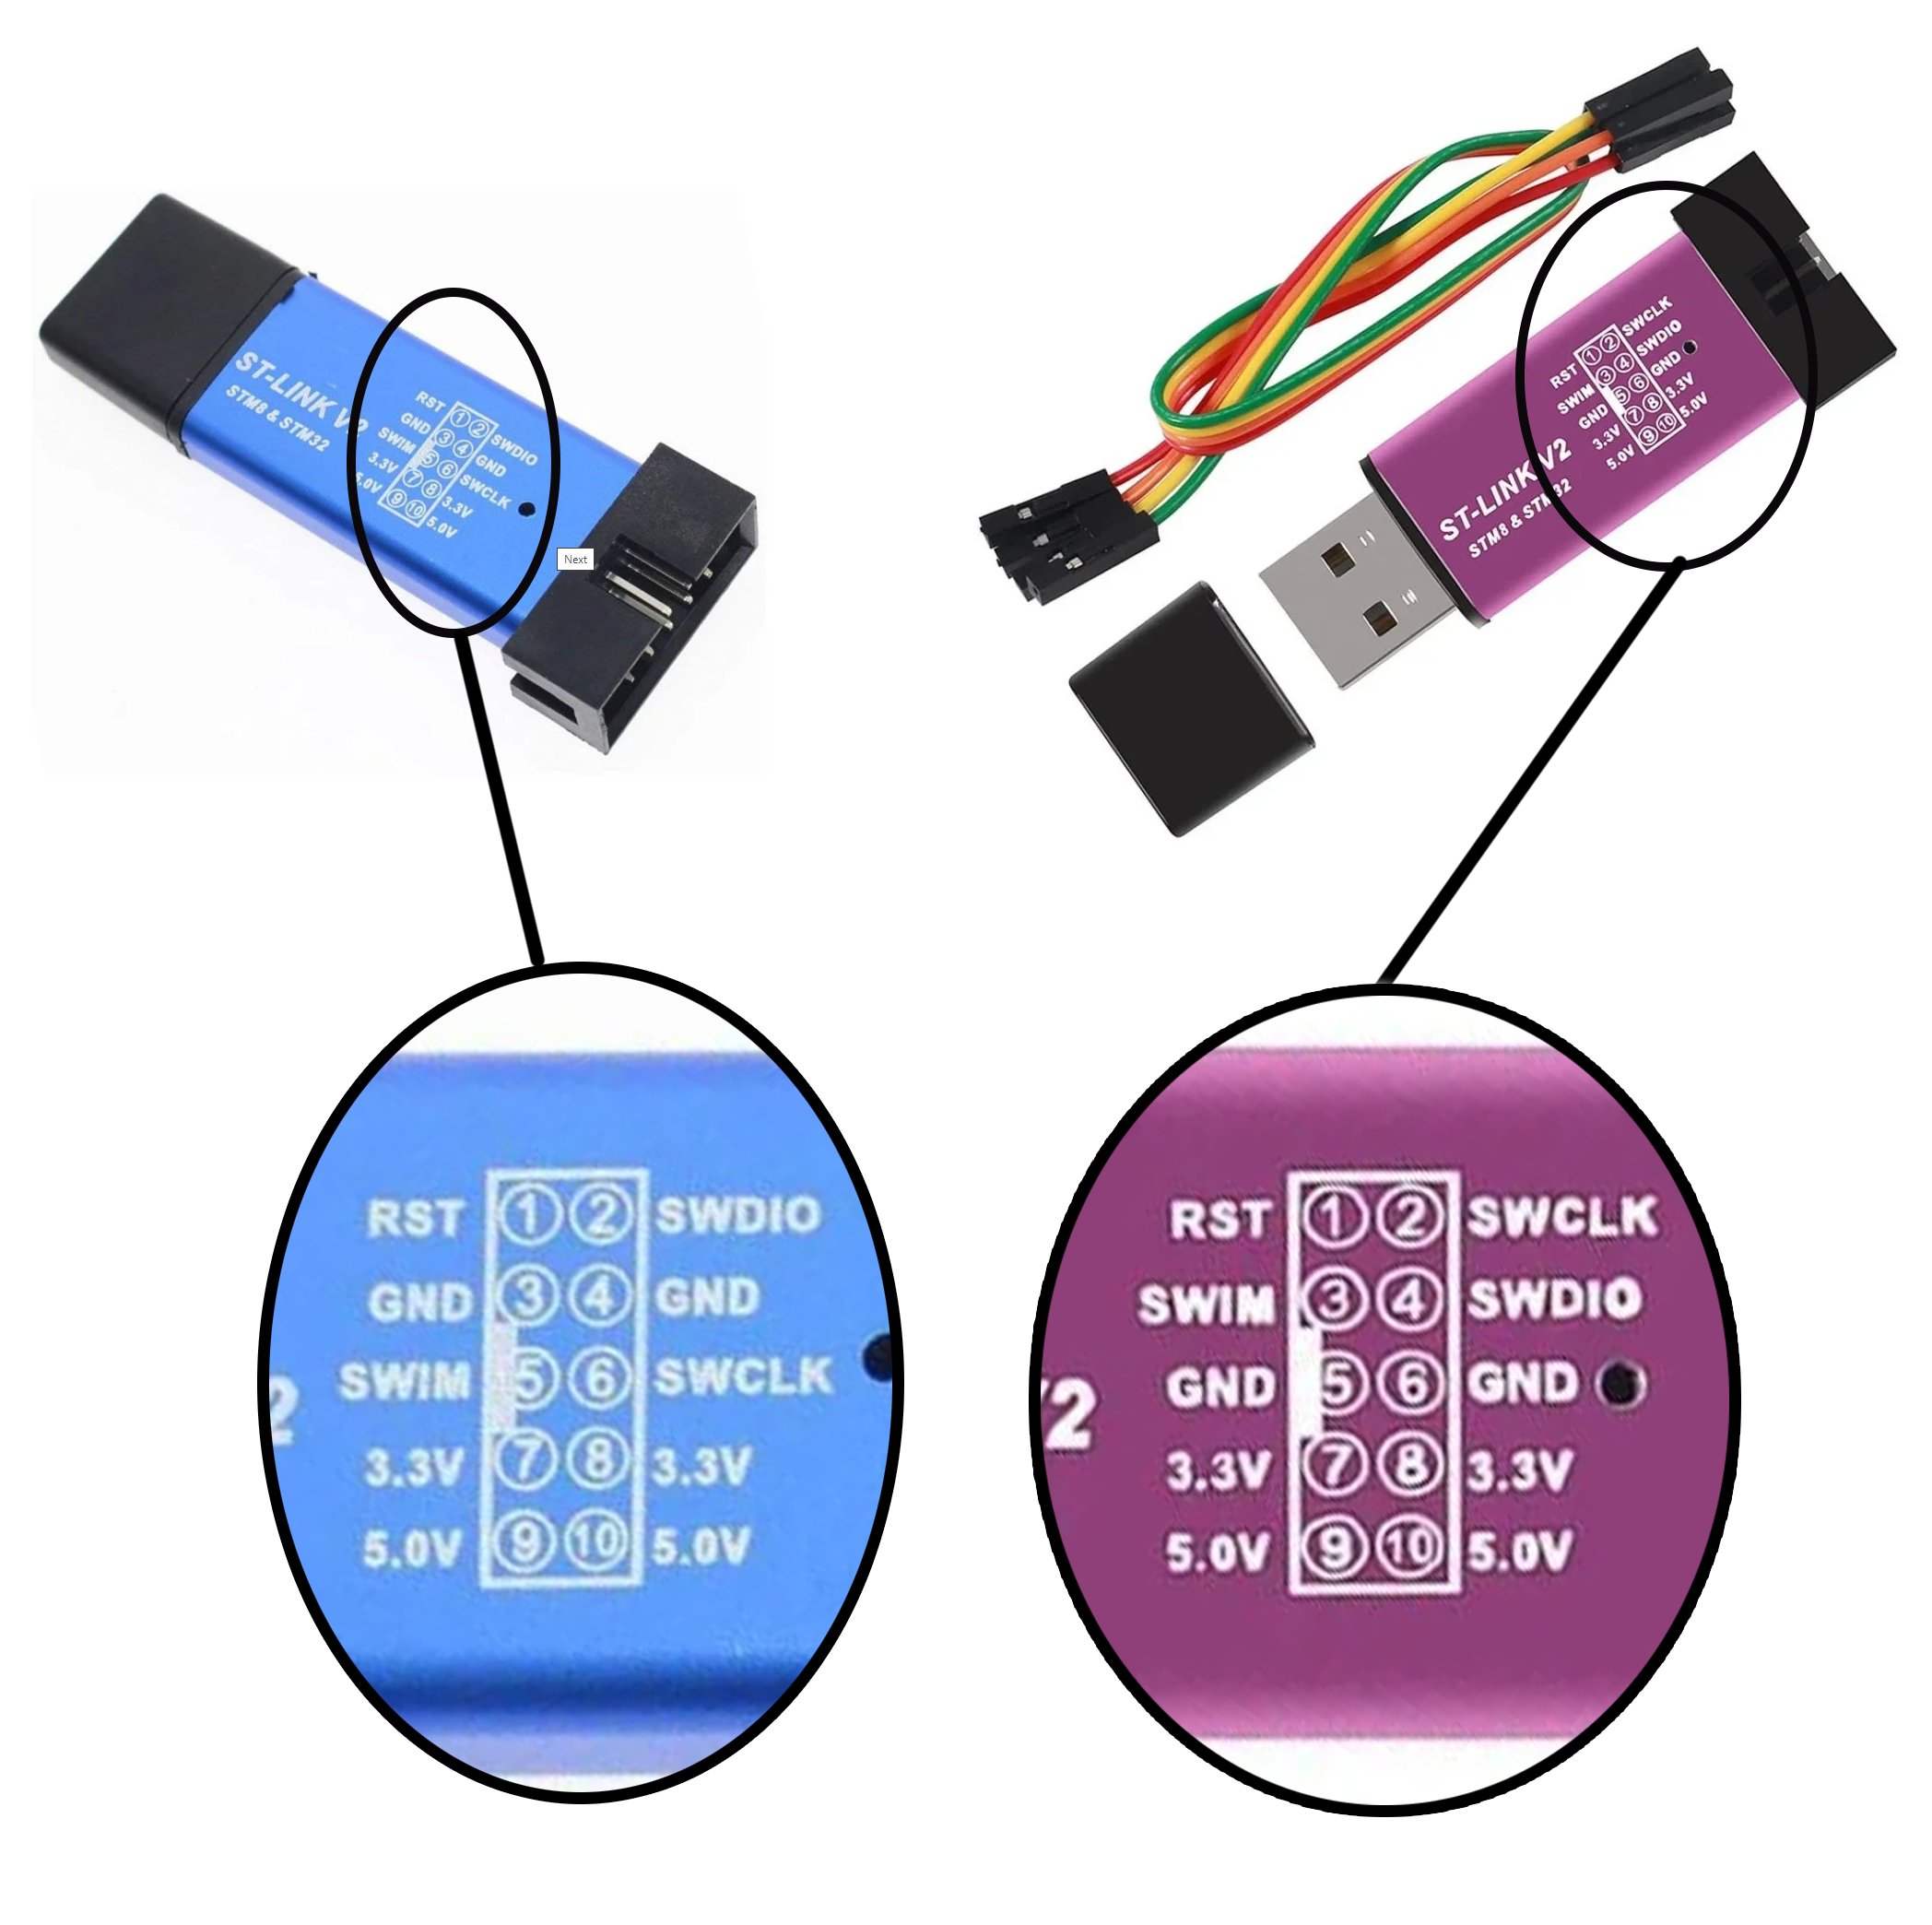
\includegraphics[width=0.5\textwidth]{figures/stlinkv2_cheap_pin_diff}
	\caption{St-Link V2 paralelo e o problema da não padronização de pinos}
    \label{stlinkv2_cheap}
\end{figure}





\subsection{ESP32 Devkit v1}




% ESP32 Series
% core = ESP32-D0WD-V3
% ESP32-WROOM-32E - https://www.espressif.com/sites/default/files/documentation/esp32-wroom-32e_esp32-wroom-32ue_datasheet_en.pdf

% https://olddocs.zerynth.com/r2.4.2/official/board.zerynth.doit_esp32/docs/index.html





\section{IDE}

\subsection{Atollic TrueSTUDIO}

A IDE a ser usada para programar um STM32 seria o TrueSTUDIO, distribuído pela
Atollic, que foi adquirida pela STMicroelectronics em 2017. Trata-se de um
software livre para programar em C/C++, criado com base na plataforma Eclipse,
e que possui todas as funções esperadas para o trabalho com o STM32, tais como
edição, compilação e debugging. Uma de seus principais vantagens é não haver
limites para tamanho de projeto, o que o torna ideal para trabalhos
profissionais. O TrueSTUDIO deixou de receber atualizações em 2017,
depois da aquisição pela STMicroelectronics.\cite{apostila_microprossados}

\begin{figure}[ht]
	\centering
	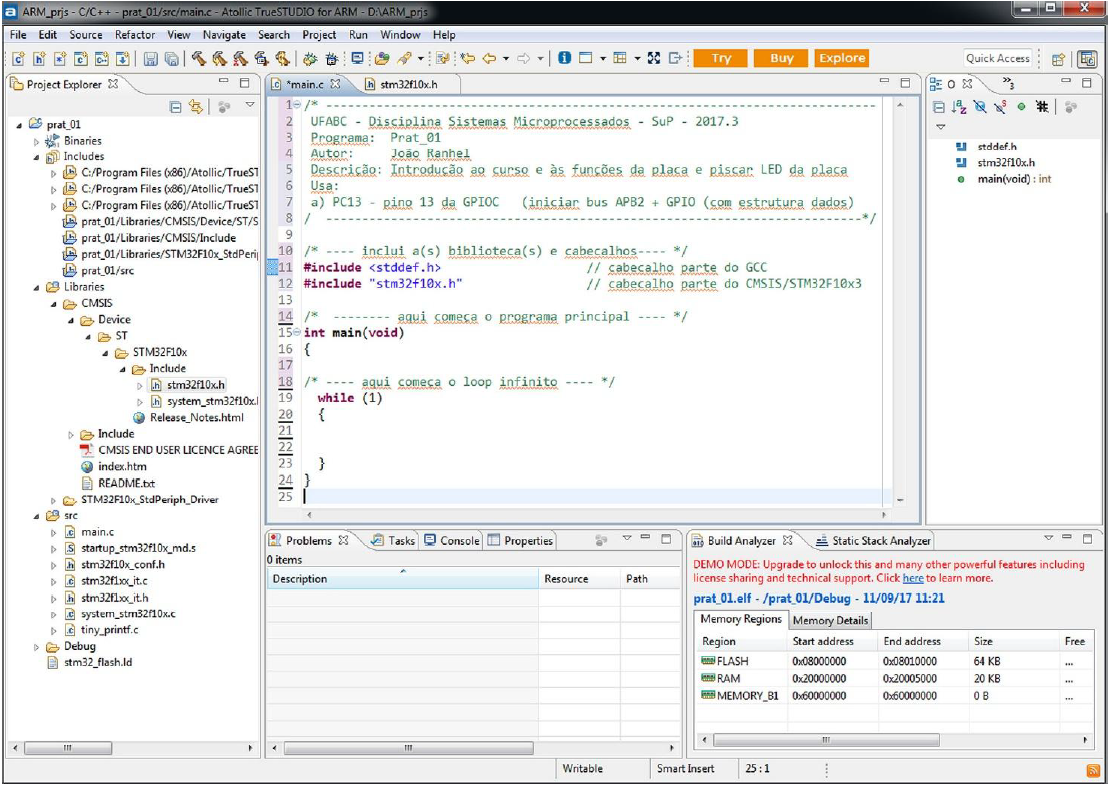
\includegraphics[width=0.8\textwidth]{figures/atollic}
	\caption{Interface Atollic \cite{apostila_microprossados}}
\end{figure}


\subsection{Arduino}
Devido a complicações nas configurações de múltiplas saídas de PWM com o
TrueSTUDIO, optou-se por usar Arduino como alternativa. Um obstáculo a essa
alternativa é que o Arduino não é compatível com STM32 nativamente, porém um
o projeto STM32duino \cite{STM32duino}, criado por Frédéric Pillon, engenheiro
de software na STMicroelectronics \cite{fpistm}, permite instalar a bibliotecas
do STM32 no Arduino. No momento de escrita deste trabalho, o projeto era
compatível apenas com a versão 1.8 da IDE do Arduino.

\begin{figure}[ht]
	\centering
	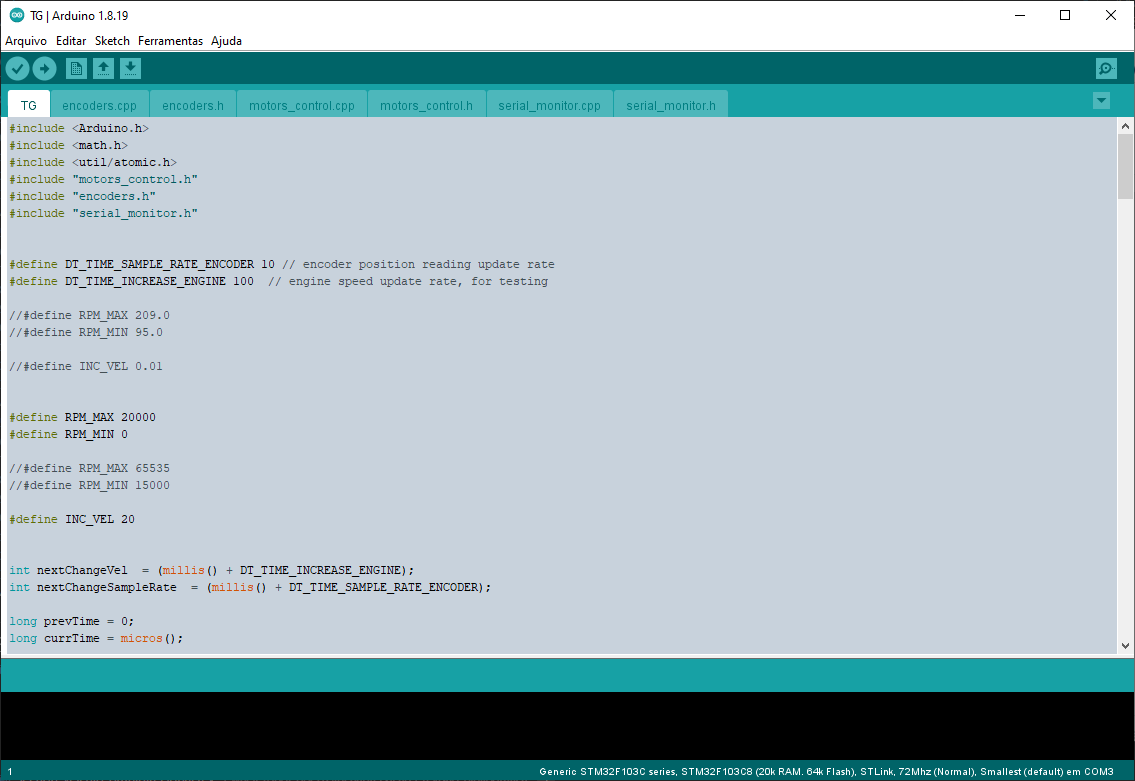
\includegraphics[width=1\textwidth]{figures/arduino}
	\caption{Interface Arduino}
\end{figure}




\section{CAD - Design auxiliado por computador}
CAD é a sigla para "computer-aided design", design auxiliado por computador, e pode ser definido como o uso de sistemas computadorizados (hardware + software)
para criação, modificação, análise ou otimização do design \cite{computer_aided_esign}.
O software CAD consiste em um programa capaz de implementar gráficos computadorizados e aplicar funções como análise tensão-deformação de componentes, resposta dinâmica de mecanismos,
cálculos de transferência de calor. As aplicações variam conforme a necessidade da área.

\subsection{AutoCAD}
AutoCAD foi criado em 1982, seu uso mais popular é em desenhos arquitetônicos, mas também tem um forte uso na criação de desenhos técnicos.

\begin{figure}[h]
	\centering
	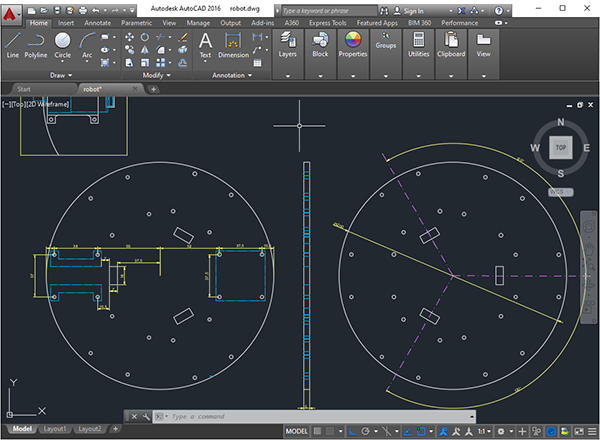
\includegraphics[width=1\textwidth]{figures/autocad_screen}
	\caption{Interface do AutoCad}
	\label{fig:interface_autocad}
\end{figure}

\subsection{SolidWorks CAD 3D}
Com um foco maior em projetos de engenharia, esse software CAD tem um foco na criação do modelo 3D das peças, considerando precisão de medidas e materiais.
O pacote de softwares adicionais oferece simulações de elementos finitos como análise térmica, vibrações, queda, dinâmica, pressão entre outros.

\begin{figure}[h]
	\centering
	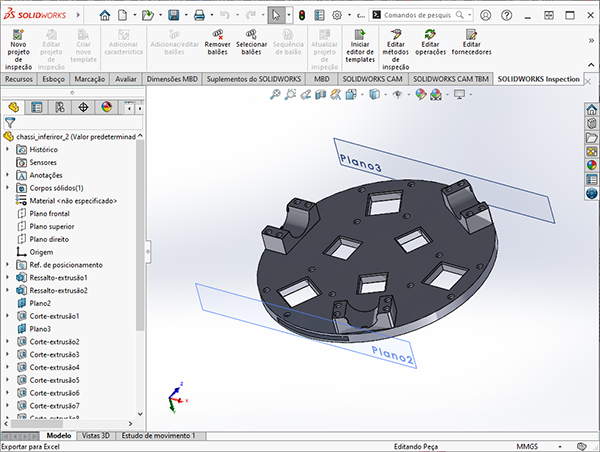
\includegraphics[width=1\textwidth]{figures/soliworks}
	\caption{Interface do SolidWorks}
	\label{fig:interface_soliwoks}
\end{figure}

\section{Impressão 3D de filamento - Manufatura Aditiva}
A manufatura aditiva é o processo de fabricação a partir de adição de camadas de materiais com base em dados de
CAD-3D \cite{manufatura_aditiva}. Manufatura aditiva é o nome que se dá para impressão 3D, se constituindo como
terceiro pilar na tecnologia de manufatura, que inclui também a "manufatura subtrativa" (mais conhecido como processos
de usinagem) e a "manufatura formativa" (como fundição, injeção e conformação).

Como ilustrado na figura \ref{fig:manufatura_aditiva}, asas etapas típicas da manufatura aditiva são:

\begin{enumerate}
	\item Obtenção do modelo CAD 3D;
	\item Fatiamento do modelo e obtenção o contorno das camadas;
	\item Adição de camadas de materiais;
	\item Obtenção do produto final.
\end{enumerate}

O modelo é fatiado por meio de um software, e o resultado é geralmente um conjunto de contornos de mesma espessura.
Esse conjunto de contornos é convertido em comandos a serem executados por uma máquina, em ações de processamento das
camadas. No caso de uma impressora 3D de filamento, o software que obtém as informações de camadas converte essas
informações em código G, linguagem padronizada para máquinas CNC.

\begin{figure}[h]
	\centering
	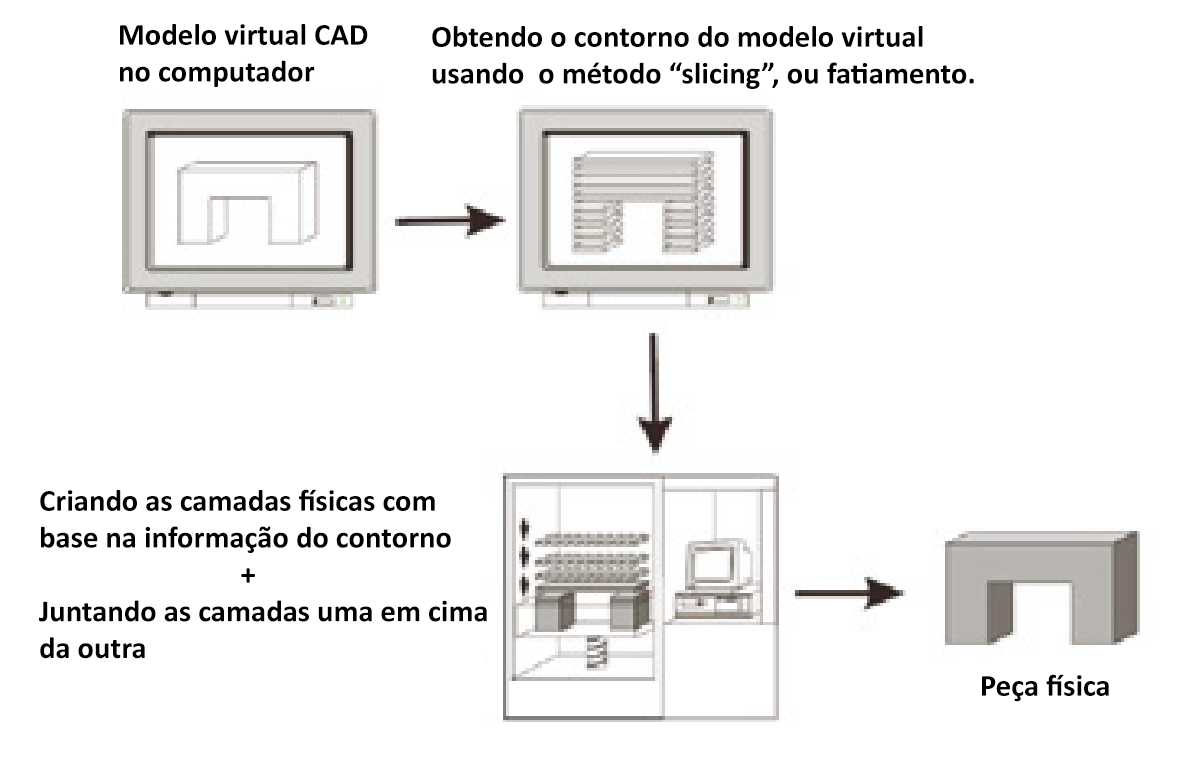
\includegraphics[width=1\textwidth]{figures/manufatura_aditiva}
	\caption{Processo de manufatura aditiva \cite{manufatura_aditiva}}
	\label{fig:manufatura_aditiva}
\end{figure}


	
\chapter{Metodologia}

{\color{red}Este capítulo dedica-se a prover uma visão geral das etapas necessárias à conclusão deste projeto, e também
permite sua eventual reprodução no futuro.}

Para a execução deste projeto, optou-se pelo uso de componentes amplamente disponíveis no mercado a relativamente baixo
custo, bem como software disponível gratuitamente no site do fabricante.


\section{Hardware}
{\color{red} Esta seção especifica os componentes físicos envolvidos no robô desenvolvido para o projeto, descrevendo
também a função de cada um no desempenho das suas funções.}
{\color{red} Inserir aqui tabela com o custo dos componentes.}

\subsection{Fabricação e montagem}
Foi decido fabricar o chassi e demais peças usando impressão 3D, com PLA.
O projeto das peças foi realizado no AutoCAD e depois modelado em 3D com SolidWorks, após a modelagem realizada,
a geometria das peças foram convertidas em código G para um impressora 3D usando o UltiMaker Cuda, a impressora usada foi a Ender 3 S1 Pro
As figuras relacionadas ao CAD, podem ser encontradas no anexo \ref{att_fabricao_montagem_cad}, quanto a modelagem,
anexo \ref{att_fabricao_montagem_modelagem}, e impressão 3D e montagem, anexo \ref{att_fabricao_montagem_impressao}.



\subsection{Motor DC e driver}
Optou-se pelo uso de um motor DC de 6V 210rpm, com taxa de redução de 1:34. O motor já possui um encoder magnético
acoplado, com 11 PPR (\textit{Pulses Per Revolution}). 
Inicialmente foi testado o driver Ponte H L298N para ligar cada motor, suporta até 2A em operação DC \cite{datasheel_l298n},
a corrente de operação máxima do motor é de 1.1A, porém a corrente de parada é drenar 3.2A. 
O L298N também causa uma queda de tensão, a 1A pode causar uma queda de 3.2V, fazendo com que o
motor não receba a tensão necessária para operar nos valores desejados \cite{datasheel_l298n}. 
O L298N é mais recomendado para tensões entre 12V a 40V, como o motor é de 6v, acaba tendo uma queda de tensão considerável.
Com isso, um driver de para baixas tensões é recomendado, foi escolhido o DRV8833 \cite{datasheel_dvr8833}.

\begin{figure}[h]
	\centering
	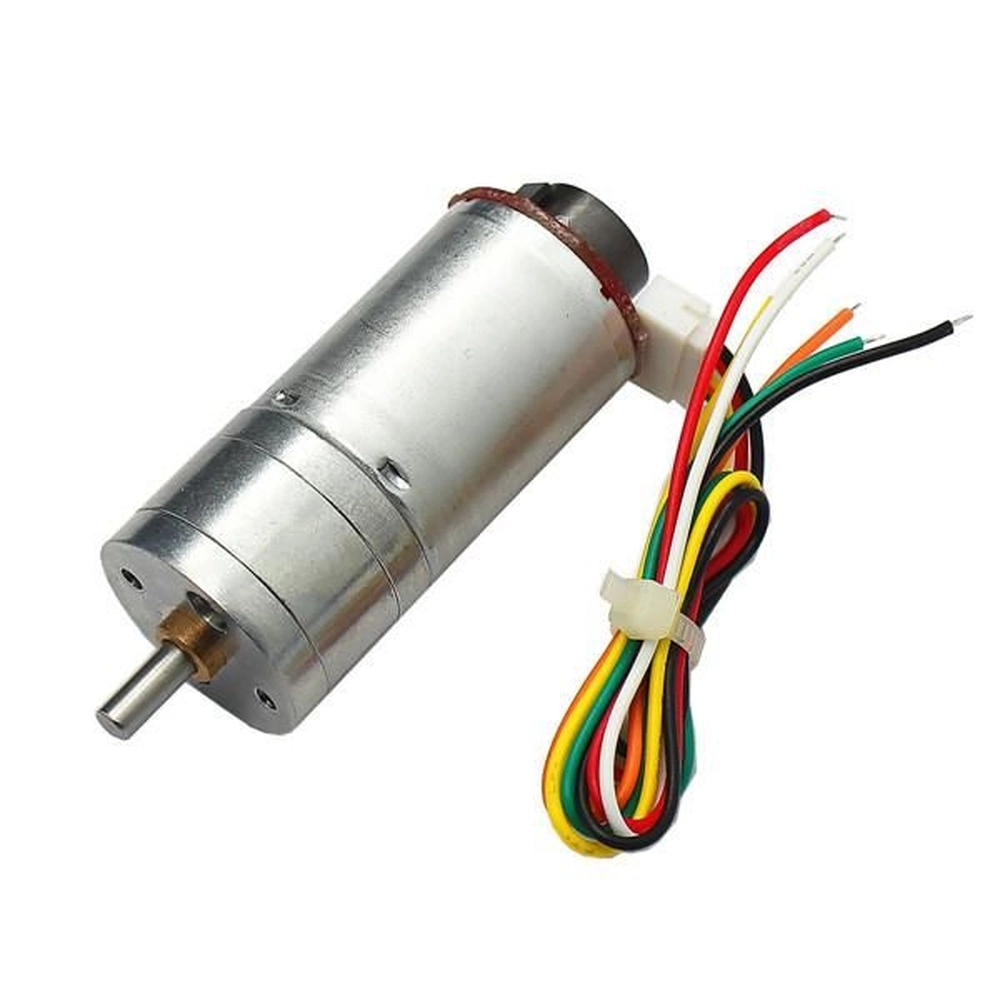
\includegraphics[width=0.7\textwidth]{figures/CHR_GM25_370}
	\caption{Motor DC 6V \cite{motor_dc_6v_encoder}}
\end{figure}


\begin{quadro}[htb]
	\caption{\label{Especificacoes_motordc_6v}Especificações do motor DC 6V}
	 \begin{tabular}{|c|c|c|c|}
		\hline
		\textbf{Componente} & \textbf{Quant} \\ \hline
		Tensão nominal & DC 6V  \\ \hline
		Velocidade sem carga  & 210RPM 0.13A  \\ \hline
		Eficiência máxima & 2,0kg.cm/170rpm/2,0W/0,60A   \\ \hline
		Poder máximo & 5,2kg.cm/110rpm/3,1W/1,10A   \\ \hline
		Torque de parada  & 10kg.cm 3.2A    \\ \hline
		Taxa de Redução do Retardador & 1:34  \\ \hline
		Resolução do salão & Razão Hall x 34,02 = 341,2PPR  \\ \hline
	\end{tabular}
	\fonte{\cite{chinhai_motor}}
	\end{quadro}

\begin{figure}[h]
	\centering
	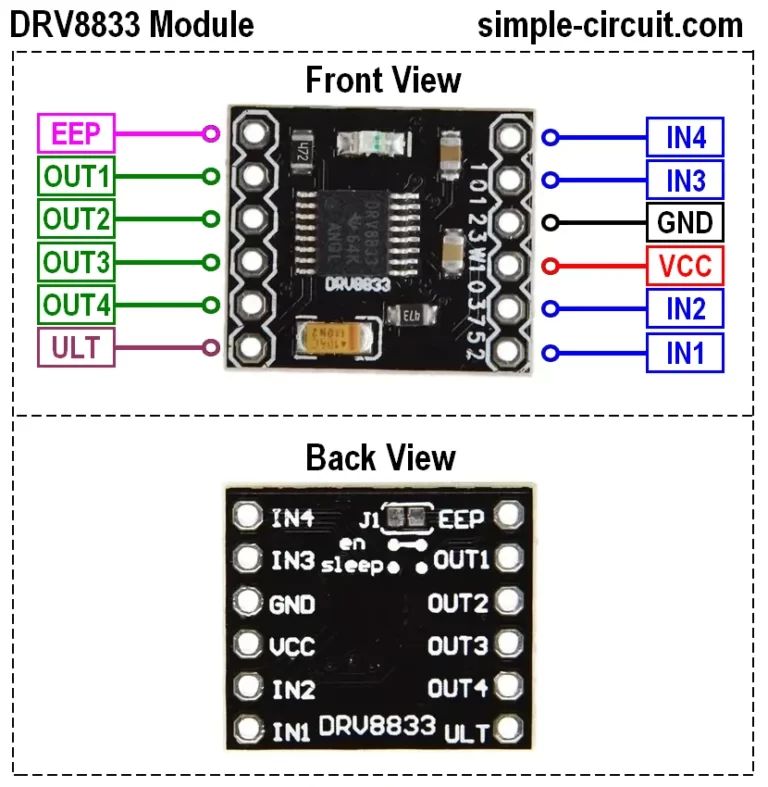
\includegraphics[width=0.7\textwidth]{figures/DRV8833-Dual-Driver-Pinout}
	\caption{Driver Ponte H DVR8833 \cite{DRV8833_image}}
\end{figure}

\subsection{Microcontrolador}

Para microcontrolador, optou-se pelo uso do  STM32F103C8, também conhecido como Blue Pill.
Possui como processador o ARM Cortex-M3, e tem 64Kbs de memória flash. 
O STM32F103C8 possui 7 timers, 2 ADCs, e 9 interfaces de comunicação, incluindo
I2C (\textit{Inter-Integrated Circuit}), USART (\textit{Universal Synchronous
Asynchronous Receiver Transmitter}), SPI (\textit{Serial Peripheral Interface}),
CAN e USB 2.0.
O STM32F103C8 possui 6 que suportam canais de PWM de 5V, e outros 8 canais de 3.3V,  e pode ser alimentado via micro
USB de 5V.

Para carregar o projeto no microcontrolador, um gravador ST-LINK USB será utilizado.

\begin{figure}[h]
	\centering
	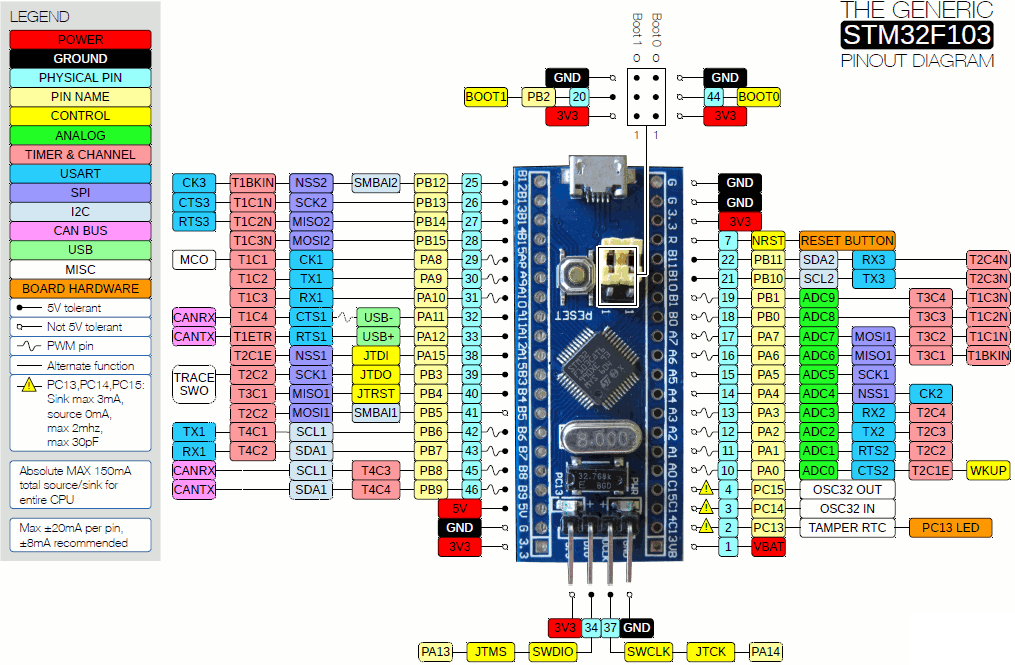
\includegraphics[width=0.8\textwidth]{figures/stm32f1_pinout}
	\caption{Diagrama de pinos do STM32F103C8}
\end{figure}

\subsection{Alimentação}
Para alimentar o microcontrolador, um powerbank com saida de 5v será usado, considerando que o STM32F103C8 funciona a
uma corrente abaixo de 100mA. Para alimentar os motores, para uso no desenvolvimento, optou-se por uma bateria de chumbo-ácido de 6V 4.5Ah

% \subsection{Joystick de controle}
% Um joystick de 3 eixos para controlar o robô para testar a cinemática de movimento.
% {\color{red} É necessário aqui especificar o modelo utilizado e descrever características.}

% \subsection{Sensores}
% {\color{red} Esta subseção deve descrever os sensores utilizados e também sua finalidade.}

% \subsection{Dispositivos de comunicação}
% {\color{red} Esta subseção deve descrever os dispositivos de comunicação utilizados (Wi-fi, Bluetooth, etc) e também sua
% finalidade.}

% \subsection{Calibração de parâmetros}
% {\color{red} Caso haja necessidade de calibração de parâmetros de alguns dos componentes utilizados (sensibilidade de
% sensores, histerese de componentes mecânicos, taxa de comunicação de dispositivos, etc), os procedimentos devem ser
% descritos nesta subseção.}

\section{Software}
{\color{red} Esta seção se dedica a discorrer a respeito dos diversos componentes de software envolvidos no projeto.}

\subsection{Controle de velocidade}

\subsubsection{Medição de velicidade do motor}

Como encoder possuí dois sinais de onda quadadra defasadas em 90º, fase A e fase B, cujos vales e picos são valores lógicos HIGH e LOW, 
e direção de rotação do motor pode ser definida pela diferença entre as fases, se fase A esta adiantada ou atrasada em relação a fase B
É possível calcular a velocidade com base nas subidas da onda quadrada de uma fase, e o valor logico da outra fase no momento da subida.
Por exemplo,  observando a fase B, toda vez em que há uma subida, se o valor da fase A for alto, então incrementar +1 em um contador, se a fase A tiver valor baixo, então incrementar -1 no contador.
Quando o valor da fase A for alto, então o motor esta rodando em um sentido,  quando o valor  for baixo, então o motor esta rodando no sentido contrário.
Medindo o valor do contador por um $\Delta_{T}$, se resulta na quantidade de pulsos por segundo.
Para converter de pulsos por segundo para RPM, basta dividir pela resolução do motor+encoder,  que é de 1:34 do motor, e 11 pulsos por rotação do encoder, o que resulta em 374,
e multiplicar por 60 para ter o resultado em rotações por minuto.

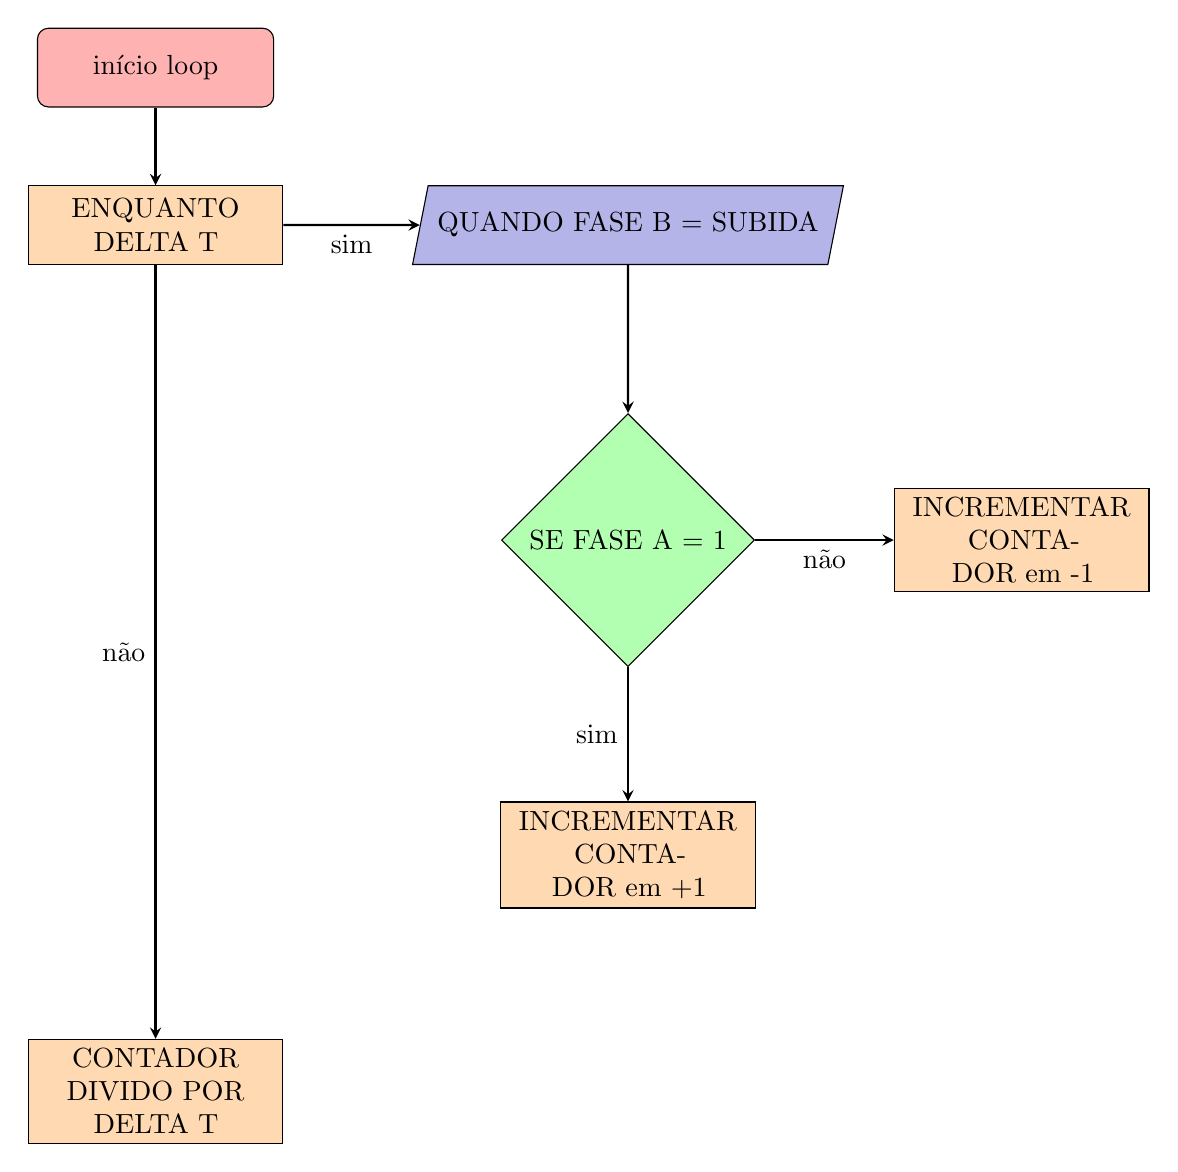
\begin{tikzpicture}[node distance=2cm]

    \node (start) [startstop] {início loop};
    \node (pro1) [process, below of=start] {ENQUANTO DELTA T};
    
    \node (in1) [io, right of=pro1, xshift= 4cm] {QUANDO FASE B = SUBIDA};
    
    \node (dec1) [decision, below of=in1, yshift=-2cm] {SE FASE A = 1};
    \node (pro1a) [process, below of=dec1, yshift= -2cm] {INCREMENTAR CONTADOR em +1};
    \node (pro1b) [process, right of=dec1, xshift= 3cm] {INCREMENTAR CONTADOR em -1};
    
    
    \node (count) [process, below of=pro1, yshift= -9cm] {CONTADOR DIVIDO POR DELTA T};
    
    \draw [arrow] (start) -- (pro1);
    \draw [arrow] (pro1) -- node[anchor=north] {sim} (in1);
    \draw [arrow] (in1) -- (dec1);
    \draw [arrow] (dec1) -- node[anchor=east] {sim} (pro1a);
    \draw [arrow] (dec1) -- node[anchor=north] {não} (pro1b);
    
    \draw [arrow] (pro1) -- node[anchor=east] {não} (count);

\end{tikzpicture}



Na implementação dessa lógica no STM32, o desafio foi a definição do $\Delta_{T}$,
Se o $\Delta_{T}$ for muito pequeno, o resultados de pulsos por segundo pode tender ao infinito, gerando valores muito altos.
Na figura \ref{fig:medidas_altas} em laranja, esta o resultado do rpm considerando o $\Delta_{T}$ como o tempo entre os ciclos do micrcontrolador.
A outra opção, foi definir um $\Delta_{T}$ fixo, definindo uma frequencia de medição pré definida, e o resultado pode ser visto em azul na figura \ref{fig:medidas_altas}
Essa outra opção de $\Delta_{T}$ resultou em um sinal que tem uma componente em alta frequência com uma amplitude até consideral.
Analisando os dois sinai no dominio da frequêcia \ref{fig:frequencia_medidas_altas}, o espectro em frequência do sinal em laranja possui amplitudes muitos semelhante em todo espectro, mas o espectro do sinal em azul, fica bem claro que em altas frequencias é composto mais por ruidos
e as frequencia médias tem amplitude menor em relação as frequências baixas, o que torna mais fácil aplicar um filtro passa-baixa para reduzir as frenquências médias e altas.

\begin{center}
    \begin{figure}
        \centering
        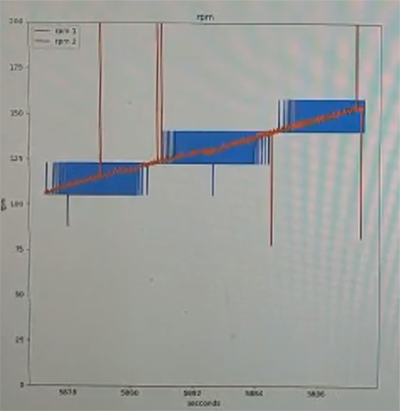
\includegraphics{figures/medidas_altas}
        \caption{Problemas com delta T muito pequeno}
        \label{fig:medidas_altas}
    \end{figure}

\end{center}

A figura \ref{fig:passa_baixa_teste}, mostra um dos teste de filtro passa baixa, em o sinal em laranja ainda persiste esses valores tentendo ao infinito, devido a ampliture eles se tornam um pouco dificil de serem retirados.
Mas o sinal em azul acaba tendo um resultado melhor depois do filtro, muito semelhando ao sinal em laranja.
Com base nesse resultado, foi decidido seguir com o método em que o $\Delta_{T}$ é definido por uma frequência pré definida.

\begin{center}
    \begin{figure}
        \centering
        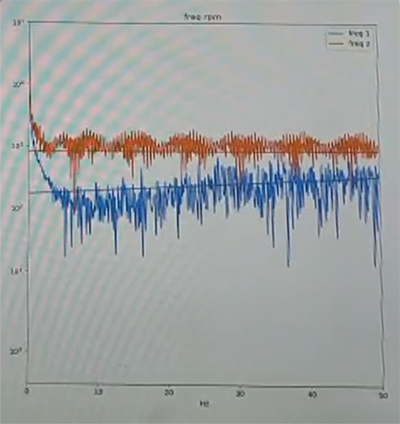
\includegraphics{figures/frequencia_medidas_altas}
        \caption{Frequências}
        \label{fig:frequencia_medidas_altas}
    \end{figure}

    \begin{figure}
        \centering
        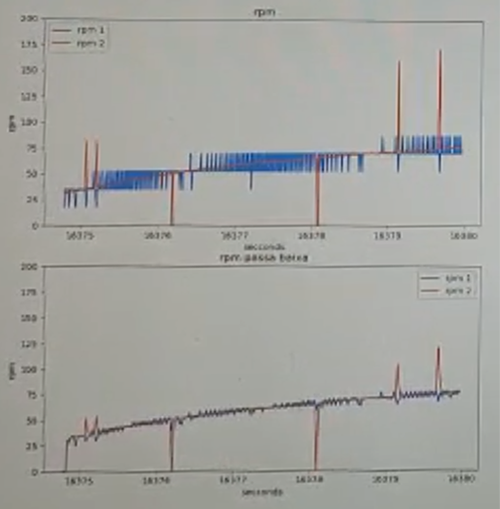
\includegraphics{figures/passa_baixa_teste}
        \caption{Passa baixa teste}
        \label{fig:passa_baixa_teste}
    \end{figure}
\end{center}

Com o método definido, foi definido um $\Delta_{T}$ em 100hz eu um filtro passa baixa em 2hz
As imagens no anexo \ref{att_medicao_motores}, mostra as imagens comparando o sinal original e o sinal filtrado para cada motor.
A equação \ref{eqn:equacao_diferenca} a seguir é a equação de diferença do filtro, considerando uma amostragem de 100hz e frequência de corte em 2hz.

\begin{equation}
    \begin{split}
        y[k] = 0.0591174 \cdot u \left[ k \right] +  0.0591174 \cdot u[k - 1] + 0.88176521 \cdot y[k - 1]
    \end{split}
    \label{eqn:equacao_diferenca}
\end{equation}

\subsubsection{Curva PWM x RPM - problema da não linearidade}

Depois de definido como calcular a velocidade o prózimo desafio foi lidar com a não linearidade entre o PWM e o resultado medido em RPM.

\begin{figure}[p]
	\centering
	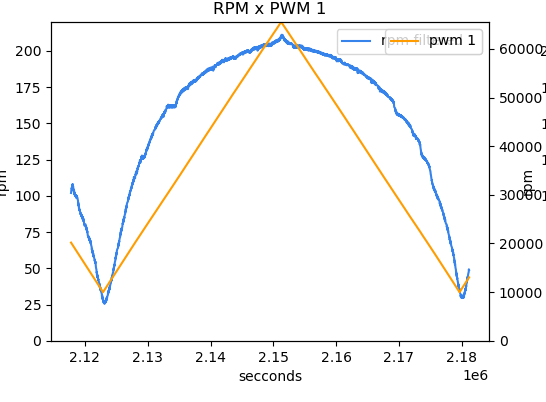
\includegraphics{figures/pwm_x_rpm}
	\caption{Curva PWM e RPM no tempo}
	\label{fig:grafico_pwm_x_rpm}
\end{figure}

Considerando essa não linearidade, foram realizadas 15k medições em PWM vs RPM para definir uma equação que pudesse relacionar o PWM com o RPM.

\begin{figure}[p]
	\centering
	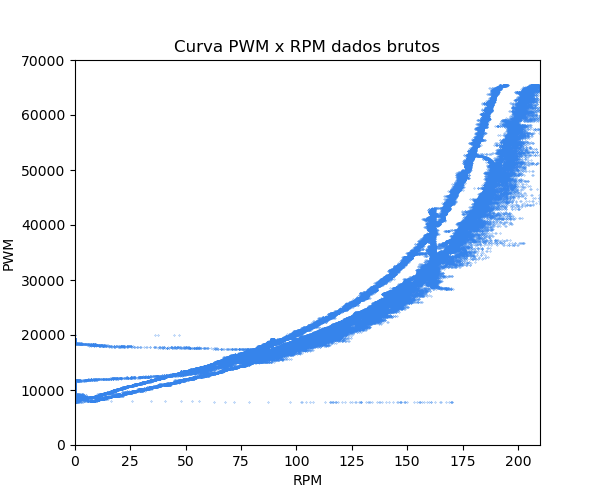
\includegraphics{figures/curva_pwm_x_rpm_dados_brutos}
	\caption{Curva PWM x RPM dados brutos}
	\label{fig:medicao_pwm_x_rpm_dados_brutos}
\end{figure}


Limpeza dos dados realizada no python
\lstset{language=Python}
\begin{lstlisting}
    import json
    import pandas as pd
    import numpy as np
    import matplotlib.pyplot as plt
    
    res = open('mediadas_capturadas.txt').read()
    res = res.split('\n')
    
    res = [json.loads(i[i.find('''{"millis":'''):]) for i in res]
    
    dados_brutos = pd.DataFrame(res)
    
    dados_brutos = pd.concat([
        dados_brutos[['w1','filterRpm_1']]
        .rename(columns={'filterRpm_1':'filter_rpm_','w1':'w'}),
        dados_brutos[['w2','filterRpm_2']]
        .rename(columns={'filterRpm_2':'filter_rpm_','w2':'w'}),
        dados_brutos[['w3','filterRpm_3']]
        .rename(columns={'filterRpm_3':'filter_rpm_','w3':'w'})
    ]).sort_values('w')
    
    
    dados_medios = dados_brutos.groupby('w').agg({
        'filter_rpm_':['mean']
    }).reset_index()
    
    
    dados_medios.columns = [''.join(i) for i in dados_medios.columns]
    
    dados_medios['cut'] = (dados_medios['w']/200).astype(int)
    dados_medios_amostra = dados_medios.groupby('cut').first().reset_index()
    
    dados_medios_amostra[
        ['filter_rpm_mean', 'w']
    ].to_csv('amostra_invertida.csv', index=False)

\end{lstlisting}


\begin{figure}[p]
	\centering
	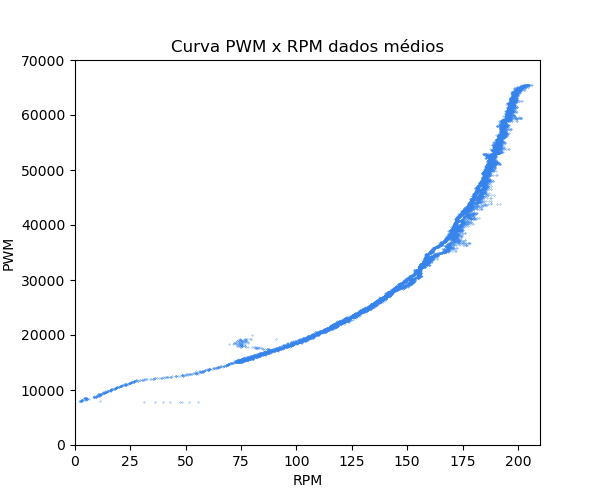
\includegraphics{figures/curva_pwm_x_rpm_dados_medios}
	\caption{Curva PWM x RPM dados médios}
	\label{fig:medicao_pwm_x_rpm_dados_medios}
\end{figure}


Matlab
\lstset{language=Matlab}
\begin{lstlisting}
    T = readtable('amostra_invertida.csv');
    filter_rpm_mean =  T{:,1};
    w =  T{:,2};
    f=fit(filter_rpm_mean,w,'poly4')

    f = 
    
         Linear model Poly4:
         f(x) = p1*x^4 + p2*x^3 + p3*x^2 + p4*x + p5
         Coefficients (with 0.95 confidence bounds):
           p1 =   0.0001131  (9.732e-05, 0.0001288)
           p2 =    -0.03064  (-0.0375, -0.02377)
           p3 =       2.993  (1.999, 3.988)
           p4 =      -1.257  (-54.15, 51.63)
           p5 =        9017  (8235, 9798)

\end{lstlisting}

\begin{figure}[p]
	\centering
	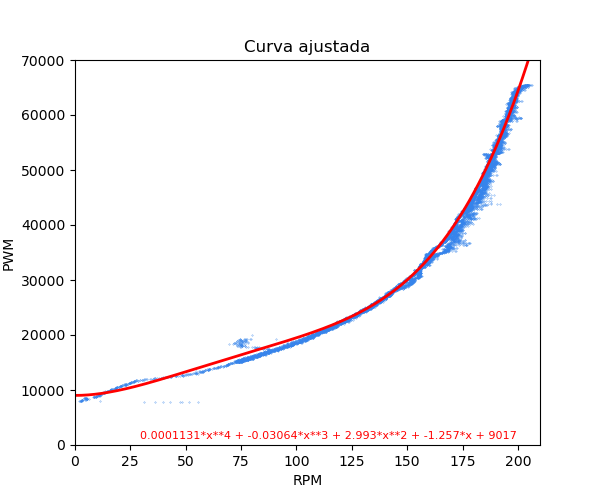
\includegraphics{figures/curva_ajustada}
	\caption{Curva ajustada}
	\label{fig:curva_ajustada}
\end{figure}


Polinônio da curva

\begin{equation}
    \begin{split}
        0.0001131x^{4} + -0.03064x^{3} + 2.993x^{2} + -1.257x + 9017
    \end{split}
\end{equation}



\subsection{Controle de posição}
{\color{red} Esta subseção deve descrever como controlar a posição do robô no ambiente interno - presumivelmente, por
meio de sensores e alguma lógica de posicionamento.}

\section{Mapeamento de ambiente}
{\color{red} O objetivo desta seção é descrever a abordagem para mapeamento de ambientes internos - seja carregando um
mapa a partir de coordenadas, ou qualquer outra abordagem adotada.}
	
	

\chapter{Desenvolvimento}


\subsection{Montagem da parte elétrica}

Os componentes foram ligados usando cabos do tipo jumper e protoboard para encaixar o microcontrolador e os drivers,
essa ligação foi útil para realizar os testes, porém o uso cabos do tipo jumper e protoboard podem oferecer mau contado, causando falhas no funcionamento do robô.
Para realizar testes finais, realizar junção dos cabos, e soldar os cabos a conectores JST devem resolver o problema de mau contado.


\subsubsection{Ligação dos componentes}
Cada motor precisa de 2 sinais de PWM, então foi necessário usar 6 pinos de PWM do STM32, as duplas de pinos que suportam PWM foram $P_{B6}$ - $P_{B7}$, $P_{B8}$ - $P_{B9}$ e $P_{A9}$ - $P_{A10}$, respectivamente para os motores 1, 2 e 3
E para cada encorder de motor, foi necessário mais 6 pinos, 2 pinos para cada fase dos 3 encoders, $P_{B0}$ - $P_{B1}$, $P_{A6}$ - $P_{B7}$ e $P_{B10}$ - $P_{B11}$, também respectivamente para os motores 1, 2 e 3, sendo os  $P_{B1}$, $P_{B7}$ e $P_{B11}$ definidos para a Fase A do encoder
A alimentação dos encoders será feito pelo pino de 3.3v do STM32, e o GND também vindo do microcontrolador.
O Módulo bluetooth HC-05 terá alimentação sendo fornecida pelo pino de 5v do microtrolador (GND sendo o mesmo usado para os encoders).
Já a comunicação serial será feita conectando o TXD do módulo com o pino $P_{A3}$, que é o pino RX2 (RX da $USART\_2$), e o RXD do módulo conectado ao $P_{A2}$, pino TX2 (TX da $USART\_2$).
Embora o HC-05 trabalhe com UART, o protocolo USART é compatível com UART, podendo usar os pinos de uma USART como se fossem uma UART.

Os pinos de PWM são conectados nos drivers DVR8833, com  $P_{B6}$, $P_{B8}$ e $P_{A9}$ como inputs nos pinos $IN1$ de cada driver, e os demais pinos conectados aos pinos $IN2$.
A alimentação dos drivers é feita por uma fonte de 6v, e os pinos $OUT1$ e $OUT2$ dos drivers conectados respectivamente as entradas $M1$ e $M2$ dos motores. A figura \ref{fig:diagrama_montagem} contém o diagrama com as ligações descritas.

\begin{figure}[htb]
	\centering
	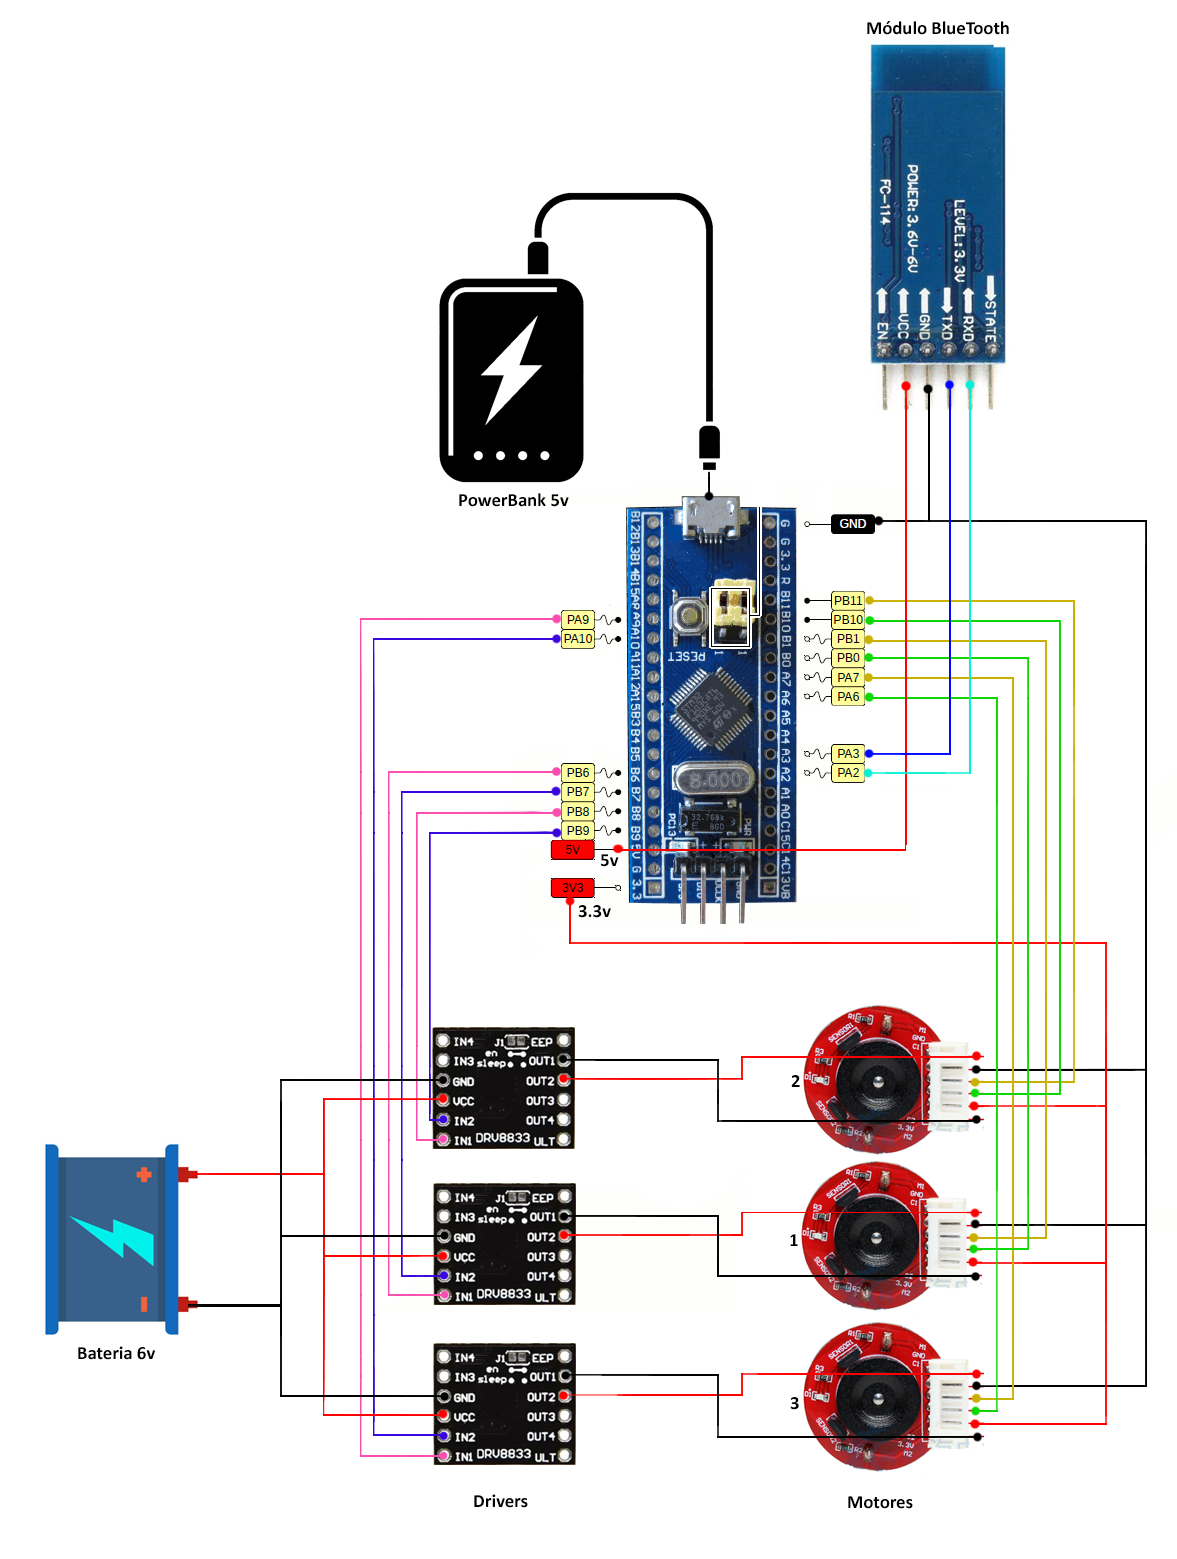
\includegraphics[width=1.0\textwidth]{figures/diagrama_montagem}
	\caption{Diagrama de montagem dos componentes}
	\label{fig:diagrama_montagem}
\end{figure}


\subsubsection{Modelagem e fabricação da estrutura}

O desenvolvimento das peças usadas na estrutura do robô foram feitas usando AutoCAD, o chassi principal que possui a geometria circular do robô foi desenhado com base nas medidas finais do robô,
com foco no raio até o centro das rodas, o raio planejado é de 100mm. Os mancais foram planejados com base nas dimensões dos motores. 

As figuras relacionadas ao CAD, podem ser encontradas no anexo \ref{att_fabricao_montagem_cad}, quanto a modelagem,
anexo \ref{att_fabricao_montagem_modelagem}, e impressão 3D e montagem, anexo \ref{att_fabricao_montagem_impressao}.



\subsection{Controle de velocidade}

\subsubsection{Medição de velicidade do motor}

Como encoder possuí dois sinais de onda quadadra defasadas em 90º, fase A e fase B, cujos vales e picos são valores lógicos HIGH e LOW, 
e direção de rotação do motor pode ser definida pela diferença entre as fases, se fase A esta adiantada ou atrasada em relação a fase B
É possível calcular a velocidade com base nas subidas da onda quadrada de uma fase, e o valor logico da outra fase no momento da subida.
Por exemplo,  observando a fase B, toda vez em que há uma subida, se o valor da fase A for alto, então incrementar +1 em um contador, se a fase A tiver valor baixo, então incrementar -1 no contador.
Quando o valor da fase A for alto, então o motor esta rodando em um sentido,  quando o valor  for baixo, então o motor esta rodando no sentido contrário.
Medindo o valor do contador por um $\Delta_{T}$, se resulta na quantidade de pulsos por segundo.
Para converter de pulsos por segundo para RPM, basta dividir pela resolução do motor+encoder,  que é de 1:34 do motor, e 11 pulsos por rotação do encoder, o que resulta em 374,
e multiplicar por 60 para ter o resultado em rotações por minuto.

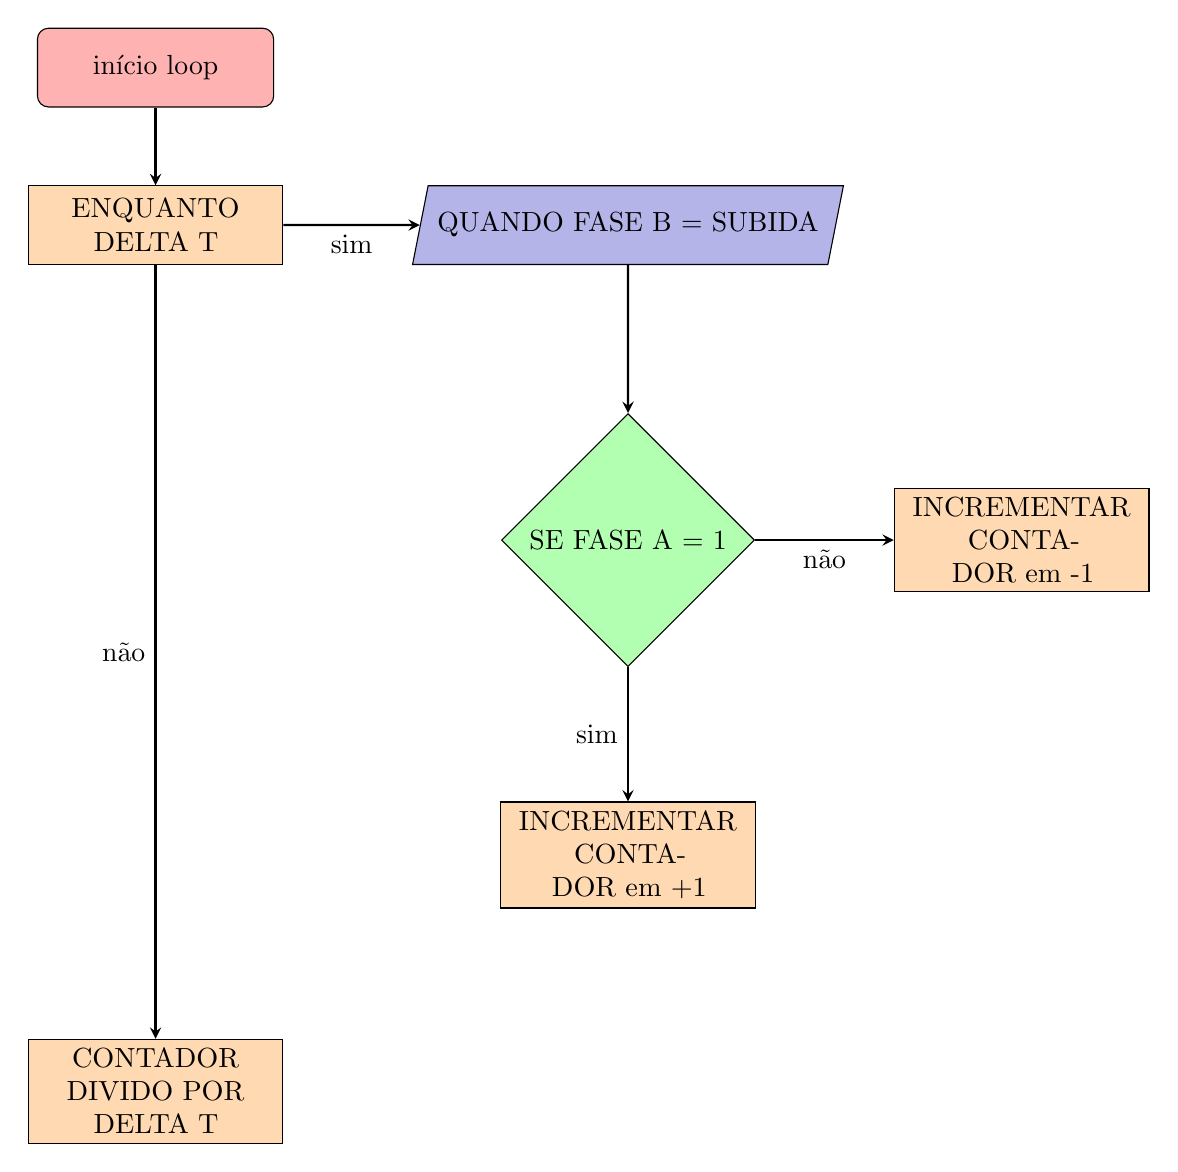
\begin{tikzpicture}[node distance=2cm]

    \node (start) [startstop] {início loop};
    \node (pro1) [process, below of=start] {ENQUANTO DELTA T};
    
    \node (in1) [io, right of=pro1, xshift= 4cm] {QUANDO FASE B = SUBIDA};
    
    \node (dec1) [decision, below of=in1, yshift=-2cm] {SE FASE A = 1};
    \node (pro1a) [process, below of=dec1, yshift= -2cm] {INCREMENTAR CONTADOR em +1};
    \node (pro1b) [process, right of=dec1, xshift= 3cm] {INCREMENTAR CONTADOR em -1};
    
    
    \node (count) [process, below of=pro1, yshift= -9cm] {CONTADOR DIVIDO POR DELTA T};
    
    \draw [arrow] (start) -- (pro1);
    \draw [arrow] (pro1) -- node[anchor=north] {sim} (in1);
    \draw [arrow] (in1) -- (dec1);
    \draw [arrow] (dec1) -- node[anchor=east] {sim} (pro1a);
    \draw [arrow] (dec1) -- node[anchor=north] {não} (pro1b);
    
    \draw [arrow] (pro1) -- node[anchor=east] {não} (count);

\end{tikzpicture}



Na implementação dessa lógica no STM32, o desafio foi a definição do $\Delta_{T}$,
Se o $\Delta_{T}$ for muito pequeno, o resultados de pulsos por segundo pode tender ao infinito, gerando valores muito altos.
Na figura \ref{fig:medidas_altas} em laranja, esta o resultado do rpm considerando o $\Delta_{T}$ como o tempo entre os ciclos do micrcontrolador.
A outra opção, foi definir um $\Delta_{T}$ fixo, definindo uma frequencia de medição pré definida, e o resultado pode ser visto em azul na figura \ref{fig:medidas_altas}
Essa outra opção de $\Delta_{T}$ resultou em um sinal que tem uma componente em alta frequência com uma amplitude até consideral.
Analisando os dois sinais no dominio da frequêcia na figura \ref{fig:frequencia_medidas_altas}, o espectro em frequência do sinal em laranja possui amplitudes muitos semelhante em todo espectro, mas o espectro do sinal em azul, fica bem claro que em altas frequencias é composto mais por ruidos
e as frequencia médias tem amplitude menor em relação as frequências baixas, o que torna mais fácil aplicar um filtro passa-baixa para reduzir as frenquências médias e altas.

A figura \ref{fig:passa_baixa_teste}, mostra um dos teste de filtro passa baixa, em o sinal em laranja ainda persiste esses valores tentendo ao infinito, devido a ampliture eles se tornam um pouco dificil de serem retirados.
Mas o sinal em azul acaba tendo um resultado melhor depois do filtro, muito semelhando ao sinal em laranja.
Com base nesse resultado, foi decidido seguir com o método em que o $\Delta_{T}$ é definido por uma frequência pré definida.


\begin{figure}[h]
    \centering
    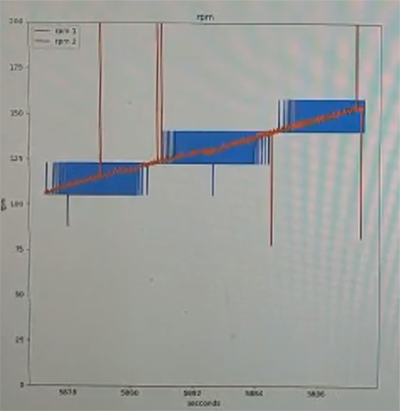
\includegraphics{figures/medidas_altas}
    \caption{Problemas com delta T muito pequeno}
    \label{fig:medidas_altas}
\end{figure}

\begin{figure}[h]
    \centering
    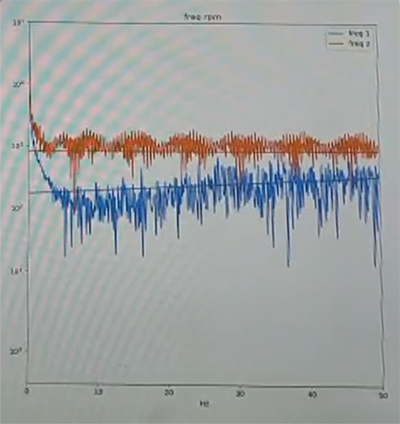
\includegraphics{figures/frequencia_medidas_altas}
    \caption{Frequências}
    \label{fig:frequencia_medidas_altas}
\end{figure}

\begin{figure}[h]
    \centering
    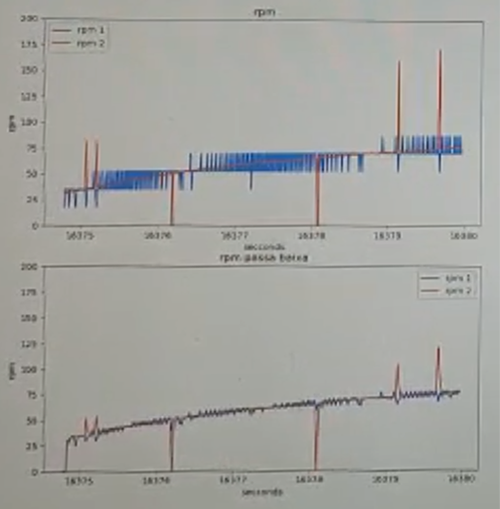
\includegraphics{figures/passa_baixa_teste}
    \caption{Passa baixa teste}
    \label{fig:passa_baixa_teste}
\end{figure}


Com o método definido, foi definido um $\Delta_{T}$ em 100hz eu um filtro passa baixa em 2hz
As imagens no anexo \ref{att_medicao_motores}, mostra as imagens comparando o sinal original e o sinal filtrado para cada motor.
A equação \ref{eqn:equacao_diferenca} a seguir é a equação de diferença do filtro, considerando uma amostragem de 100hz e frequência de corte em 2hz.

\begin{equation}
    \begin{split}
        y[k] = 0.0591174 \cdot u \left[ k \right] +  0.0591174 \cdot u[k - 1] + 0.88176521 \cdot y[k - 1]
    \end{split}
    \label{eqn:equacao_diferenca}
\end{equation}

\subsubsection{Curva PWM x RPM - problema da não linearidade}

Depois de definido como calcular a velocidade o próximo desafio foi lidar com a não linearidade entre o PWM e o resultado medido em RPM.
Como pode ser visto na figura \ref{fig:grafico_pwm_x_rpm}, na comparação entre o valor do PWM e o RPM no tempo.

\begin{figure}[htb]
	\centering
	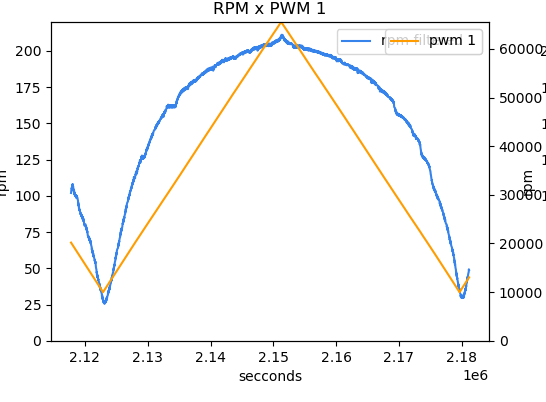
\includegraphics{figures/pwm_x_rpm}
	\caption{Curva PWM e RPM no tempo}
	\label{fig:grafico_pwm_x_rpm}
\end{figure}

Considerando essa não linearidade, foram realizadas 15k medições em PWM vs RPM para definir uma equação que pudesse relacionar o PWM com o RPM.
Como pode ser observado na figura  \ref{fig:medicao_pwm_x_rpm_dados_brutos}, os resultados possuem uma tendência, mas possuem alguns pontos fora da curta.
devido ao esses ruídos nas medições ss dados foram tratatos para obter valores médios dos resultados usando python,
o código pode ser visto no anexo \ref{att_limpeza_python}.

\begin{figure}[htb]
	\centering
	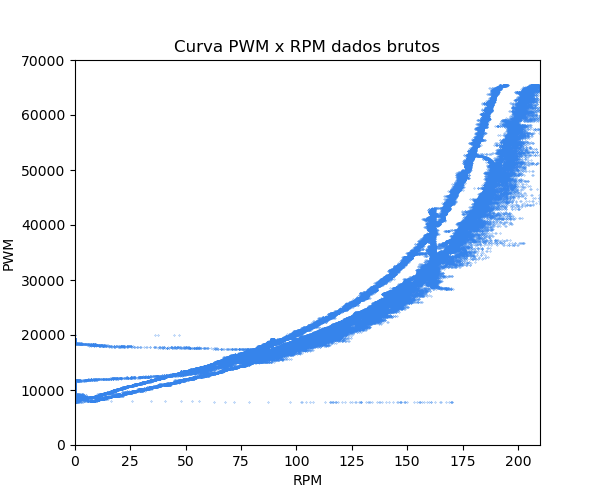
\includegraphics{figures/curva_pwm_x_rpm_dados_brutos}
	\caption{Curva PWM x RPM dados brutos}
	\label{fig:medicao_pwm_x_rpm_dados_brutos}
\end{figure}


O resultado da limpeza dos dados pode ser vizualiado na figura \ref{fig:medicao_pwm_x_rpm_dados_medios}.
Após a limpeza dos dados, os dados foram importados para o matlab, anexo \ref{att_matlab},
para obter um polinômio que possa definir a curva, o polinômio resultante é a equação \ref{eqn:polimonio_rpm}, e a figura \ref{fig:curva_ajustada} representa a curva ajustada.
A equação do polinômio foi inserida no código do micrcontrolador, foi testado definir um RPM de 150, e a tabela \ref{medicao_motores} trás uma amostra dos resultados dos RPMs de cada motor.
Com essa equação é mais fácil definir um comportamento linear, facilitando a aplicação de um controle PDI.

\begin{equation}
    \begin{split}
        0.0001131x^{4} + -0.03064x^{3} + 2.993x^{2} + -1.257x + 9017
    \end{split}
    \label{eqn:polimonio_rpm}
\end{equation}

\begin{figure}[htb]
	\centering
	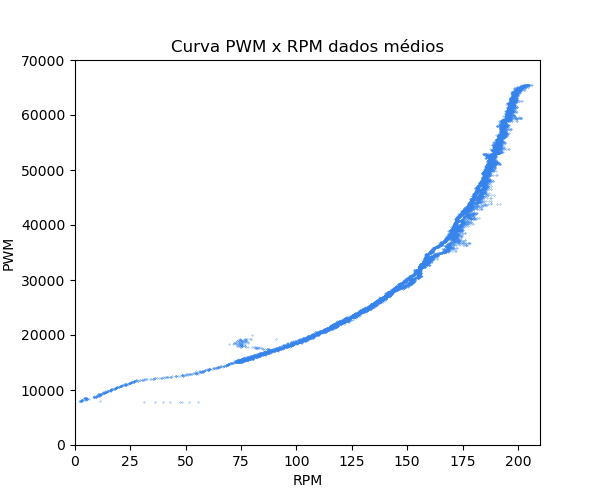
\includegraphics{figures/curva_pwm_x_rpm_dados_medios}
	\caption{Curva PWM x RPM dados médios}
	\label{fig:medicao_pwm_x_rpm_dados_medios}
\end{figure}

\begin{figure}[htb]
	\centering
	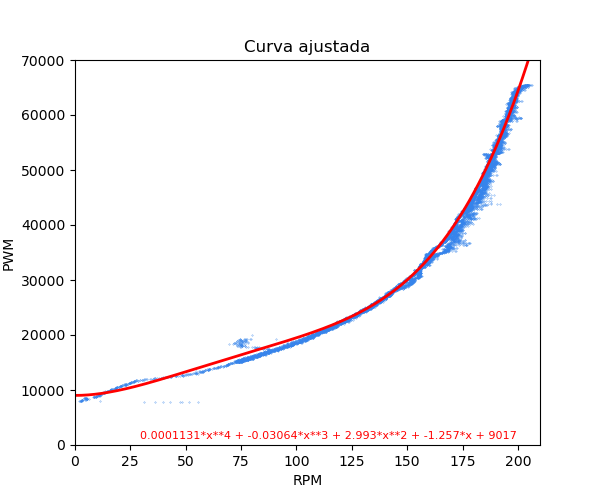
\includegraphics{figures/curva_ajustada}
	\caption{Curva ajustada}
	\label{fig:curva_ajustada}
\end{figure}



\begin{quadro}[htb]
	\caption{\label{medicao_motores}Medição rpms motores}
	 \begin{tabular}{|c|c|c|c|c|}
		\hline
		\textbf{$Tempo_{seg}$} & \textbf{$RPM_{definido}$} & \textbf{$RPM_{real_{1}}$} & \textbf{$RPM_{real_{2}}$} & \textbf{$RPM_{real_{3}}$} \\ \hline
		52.954 & 150.00  & 141.03 & 162.69 & 149.82 \\ \hline
		52.954 & 150.00  & 141.43 & 162.43 & 149.18 \\ \hline
		53.000 & 150.00  & 140.83 & 162.19 & 148.61 \\ \hline
		53.000 & 150.00  & 140.30 & 161.98 & 149.06 \\ \hline
		53.000 & 150.00  & 140.79 & 161.80 & 149.46 \\ \hline
		53.000 & 150.00  & 141.21 & 161.64 & 148.86 \\ \hline
		53.046 & 150.00  & 141.59 & 161.49 & 149.28 \\ \hline
		53.046 & 150.00  & 141.92 & 161.37 & 149.65 \\ \hline
		53.046 & 150.00  & 141.26 & 161.25 & 149.02 \\ \hline
		53.046 & 150.00  & 140.68 & 162.11 & 148.48 \\ \hline
		53.046 & 150.00  & 141.12 & 162.86 & 148.94 \\ \hline
		53.092 & 150.00  & 141.51 & 162.57 & 149.35 \\ \hline
		53.092 & 150.00  & 141.85 & 162.32 & 148.76 \\ \hline
		53.092 & 150.00  & 141.20 & 162.09 & 149.19 \\ \hline
		53.092 & 150.00  & 140.63 & 161.90 & 149.57 \\ \hline
	\end{tabular}
\end{quadro}








	

\chapter{Próximas etapas}

\section{Controle PID em motor DC}
Após lidar com o problema da não linearidade da respostado do motor ao sinal PWM
o próximo passo em controlar a velocidade é a implementação do controle PID.
O desafio será controlar a posição no tempo, considerando a velocidade resultante do robô.

\section{Integração bluetooth}
Para testar a cinematica do robô, iremos controla-lo via bluetooth. Para isso falta implementar a leitura via serial usando protocolo UART.

\section{Teste com motor de passo de alto torque - bj42d15}
Foi considerado trocar o tipo de motor e fazer um compartivo entre os diferentes tipos de controle e implementação necessário para cada tipo de motor,
e apontar as diferenças de resultados.
Foi sugerido usar o motor de passo bj42d15, comum em impressoras 3d, que possui um torque mais alto e bons resultados no uso de equipamentos que exigem precisão de posicionamento.


	% ----------------------------------------------------------
	% Finaliza a parte no bookmark do PDF
	% para que se inicie o bookmark na raiz
	% e adiciona espaço de parte no Sumário
	% ----------------------------------------------------------
	\phantompart


	% Conclusão
	%\chapter{Conclusão}
% ---

\lipsum[1]


	

% ELEMENTOS PÓS-TEXTUAIS
\postextual

	% Referências bibliográficas
	% \bibliography{abntex2-modelo-references}
	\bibliography{bibliography/bibliografia.bib}
	%\printbibliography

	% Glossário
	%%\glossary



	% Apêndices
	%\begin{apendicesenv}

% Imprime uma página indicando o início dos apêndices
% \partapendices




\chapter{Transcrição da matriz de cinemática em um bloco de código C \label{matriz_cinematica_c}}

\lstset{language=C}
\begin{lstlisting}
#include <math.h>
#define RADIUS_ROBOT 100
// mm, raio medido do centro ate o centro geometrico de cada roda
#define DEFAULT_SPEED 400 // mm/second   velocidade linear do robo.
#define RADIUS_WHEEL 34.5 //mm Raio da roda
#define PI 3.141592653589

float speedLinearToRpm(float speedLinear){
    float rpm = 60*speedLinear/(2*PI*RADIUS_WHEEL);
    return rpm;
}

void TransformationMatrixRpm(
	volatile long *w1, volatile long *w2, volatile long *w3,
	float linSpdPer, // percentagem da velocidade linear
	float dirAngle, float angSpd
){
	float linSpd_x, linSpd_y;
	linSpd_x = linSpdPer * DEFAULT_SPEED * cos(dirAngle * (PI/180));
	linSpd_y = linSpdPer * DEFAULT_SPEED * sin(dirAngle * (PI/180));

	float a1[3] = {0, -2.0/3,  RADIUS_ROBOT/3};
	float a2[3] = {1/sqrt(3), 1.0/3, RADIUS_ROBOT/3};
	float a3[3] = {-1/sqrt(3), 1.0/3, RADIUS_ROBOT/3};

	float spdLin1, spdLin2, spdLin3;
	spdLin1 = (a1[0] * linSpd_y) + (a1[1] * linSpd_x) + (a1[2] * angSpd);
	spdLin2 = (a2[0] * linSpd_y) + (a2[1] * linSpd_x) + (a2[2] * angSpd);
	spdLin3 = (a3[0] * linSpd_y) + (a3[1] * linSpd_x) + (a3[2] * angSpd);
	
	*w1 = speedLinearToRpm(spdLin1);
	*w2 = speedLinearToRpm(spdLin2);
	*w3 = speedLinearToRpm(spdLin3);	
}
\end{lstlisting}


\chapter{Transcrição da conversão de RGB para HSV em um bloco de código C \label{anx_rgb_to_hsv}}

\lstset{language=C}
\begin{lstlisting}
#include <stdio.h>
float maxOfThree(float a, float b, float c) {
	if ((a >= b) && (a >= c)) return a;
	else if ((b >= a) && (b >= c)) return b;
	else return c;
}
float minOfThree(float a, float b, float c) {
	if ((a <= b) && (a <= c)) return a;
	else if ((b <= a) && (b <= c)) return b;
	else return c;
}
void rgbToDirAngAndMag(int r, int g, int b, float *h, float *s) {
	float r_norm = r / 255.0, g_norm = g / 255.0, b_norm = b / 255.0;
	float cmax = maxOfThree(r_norm, g_norm, b_norm);
	float cmin = minOfThree(r_norm, g_norm, b_norm);
	float diff = cmax - cmin;
	if (cmax == cmin) {
		*h = 0;
	} else if (cmax == r_norm) {
		*h = fmod((60 * ((g_norm - b_norm) / diff) + 360), 360);
	} else if (cmax == g_norm) {
		*h = fmod((60 * ((b_norm - r_norm) / diff) + 120), 360);
	} else if (cmax == b_norm) {
		*h = fmod((60 * ((r_norm - g_norm) / diff) + 240), 360);
	}
	if (cmax == 0) {*s = 0;} else {*s = (diff / cmax) * 100;}
	*h = 360 - *h;
}
void main() {
	int r = 255, g = 0, b = 255; float h, s;
	rgbToDirAngAndMag(r, g, b, &h, &s);
	printf("Direction (Hue): %.2f\n", h); // res = 60
	printf("Magnitude (Saturation): %.2f\n", s); // res = 100
}
	
\end{lstlisting}
% 
\chapter{apendice 2}

\lipsum[1]


\end{apendicesenv}

	% Anexos
	%\begin{anexosenv}

% Imprime uma página indicando o início dos anexos
\partanexos

\chapter{Cálculo modelo de 3 rodas}

\begin{figure}[h]
	\centering
	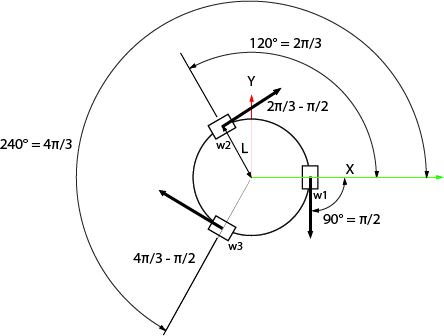
\includegraphics{figures/digram_model_dedution}
	\caption{diagrama do modelo - dedução da matriz}
	\label{lof}
\end{figure}

\begin{equation}
    \begin{split}
        \overrightarrow{V}_{l} = 
        \overrightarrow{V}_{w1}
        + \overrightarrow{V}_{w2}
        + \overrightarrow{V}_{w3}
    \end{split}
\end{equation}

\begin{equation}
    \begin{split}
        \overrightarrow{\omega} = 
        \frac{\vert\overrightarrow{V}_{w1}\vert}{L}
        + \frac{\vert\overrightarrow{V}_{w2}\vert}{L}
        + \frac{\vert\overrightarrow{V}_{w3}\vert}{L}
    \end{split}
\end{equation}


\begin{gather*}
        \dot{V}_{l} \angle \theta =  
        \dot{V}_{w1} \angle \left(-\frac{\pi}{2}\right) 
        + \dot{V}_{w2} \angle \left(\frac{2\pi}{3}-\frac{\pi}{2}\right) 
        + \dot{V}_{w3} \angle \left(\frac{4\pi}{3}-\frac{\pi}{2}\right) 
\end{gather*}

\begin{align*}
    \dot{V}_{l} \cos{ \theta } + j\dot{V}_{l} \sin{\theta} =  
    \dot{V}_{w1} \cos{ \left(-\frac{\pi}{2}\right)} + j\dot{V}_{w1} \sin{ \left(-\frac{\pi}{2}\right) } \\
    + \dot{V}_{w2}  \cos{ \left(\frac{\pi}{6}\right) } + j\dot{V}_{w2}  \sin{ \left(\frac{\pi}{6}\right) }  \\
    + \dot{V}_{w3} \cos{ \left(\frac{5\pi}{6}\right) } + j\dot{V}_{w2}  \sin{ \left(\frac{5\pi}{6}\right) } 
\end{align*}

\begin{equation*}
    \begin{split}
        \dot{\omega} = 
        \frac{\dot{V}_{w1}}{L}
        + \frac{\dot{V}_{w2}}{L}
        + \frac{\dot{V}_{w3}}{L}
    \end{split}
\end{equation*}


\begin{gather}
	\begin{bmatrix} \dot{V}\cdot \cos{\theta} \\  \dot{V}\cdot \sin{\theta} \\  \dot{\omega} \end{bmatrix}
	=
	\begin{bmatrix}
		\cos{\left(-\frac{\pi}{2}\right)} & \cos{\left(\frac{\pi}{6}\right)} & \cos{\left(\frac{5\pi}{6}\right)} \\
		\sin{\left(-\frac{\pi}{2}\right)} & \sin{\left(\frac{\pi}{6}\right)} & \sin{\left(\frac{5\pi}{6}\right)} \\
		\frac{1}{L} & \frac{1}{L} & \frac{1}{L}
	\end{bmatrix}
	\cdot
	\begin{bmatrix} \dot{V}_{w1} \\  \dot{V}_{w2} \\  \dot{V}_{w3} \end{bmatrix}
\end{gather}



\begin{gather}
	\begin{bmatrix} \dot{V}_{w1} \\  \dot{V}_{w2} \\  \dot{V}_{w3} \end{bmatrix}
	=
	\begin{bmatrix}
		0 & 2/3 & L/3 \\
		-1/\sqrt{3} & -1/3 & L/3\\
		1/\sqrt{3} & -1/3 & L/3
	\end{bmatrix}
	\cdot
	\begin{bmatrix} \dot{V}\cdot \cos{\theta} \\  \dot{V}\cdot \sin{\theta} \\  \dot{\omega} \end{bmatrix}
\end{gather}

\chapter{Outro Anexo}


\lipsum[32]



\end{anexosenv}



	

%---------------------------------------------------------------------
% INDICE REMISSIVO
%---------------------------------------------------------------------
\phantompart
\printindex


\end{document}

